% !Mode:: "TeX:UTF-8"
%% 请使用 XeLaTeX 编译本文.
\documentclass[forprint, AutoFakeBold, AutoFakeSlant ]{WHUExperiment}
%---------------------这里添加所需的命令--------------------------------
\lstdefinelanguage{json}{ % 定义json代码高亮
    morestring=[d]",
    stringstyle=\color{red!50!brown},
    showstringspaces=false,
    literate=
     *{0}{{{\color{Gray}0}}}{1}
      {1}{{{\color{Gray}1}}}{1}
      {2}{{{\color{Gray}2}}}{1}
      {3}{{{\color{Gray}3}}}{1}
      {4}{{{\color{Gray}4}}}{1}
      {5}{{{\color{Gray}5}}}{1}
      {6}{{{\color{Gray}6}}}{1}
      {7}{{{\color{Gray}7}}}{1}
      {8}{{{\color{Gray}8}}}{1}
      {9}{{{\color{Gray}9}}}{1}
      {:}{{{\color{Purple}{:}}}}{1}
      {,}{{{\color{Purple}{,}}}}{1}
      {\{}{{{\color{BlueGreen}{\{}}}}{1}
      {\}}{{{\color{BlueGreen}{\}}}}}{1}
      {[}{{{\color{BlueGreen}{[}}}}{1}
      {]}{{{\color{BlueGreen}{]}}}}{1},
}

%--------------------------------------------------------------------------
\makeatletter
\def\BState{\State\hskip-\ALG@thistlm}
\makeatother
\begin{document}
%-----------------------------------------------------------------------------

%%%%%%% 下面的内容, 据实填空.

\Ccoursename{操作系统课程设计} %课程名称
\title{操作系统课程设计} %实验名称 换行请使用\\
\author{秦槿} % 学生姓名
\Csupervisor{蒋晶珏 \quad 副教授} %指导教师一姓名、职称

% 默认不显示指导教师二,需要时可在WHUExperiment.cls 80+行处将"关闭第二指导教师显示"下一行的注释解除
\CsupervisorAnother{无} %指导教师二姓名、职称 

\CstudentNum{2021302111394} %学号
\Cmajor{计算机科学与技术} % 专业名称
\date{二〇二三年八月} % 日期

%-----------------------------------------------------------------------------

\pdfbookmark[0]{封面}{title}         % 封面页加到 pdf 书签
\maketitle
\frontmatter
\pagenumbering{Roman}              % 正文之前的页码用大写罗马字母编号.2019.6.16:更新 正文之前的页码隐藏,无需显示
%-----------------------------------------------------------------------------
% !Mode:: "TeX:UTF-8"

%%% 此部分需要自行填写: 中文摘要及关键词 

%%% 郑重声明部分无需改动

%%%---- 郑重声明 (无需改动)------------------------------------%
\newpage
\thispagestyle{empty}
\vspace*{20pt}
\begin{center}{\ziju{0.8}\pmb{\songti\zihao{2} 郑重声明}}\end{center}
\par\vspace*{30pt}
\renewcommand{\baselinestretch}{2}

{\zihao{4}%

本人呈交的设计报告,是在指导老师的指导下,独立进行实验工作所取得的成果,
所有数据、图片资料真实可靠。 尽我所知,除文中已经注明引用的内容外,
本设计报告不包含他人享有著作权的内容。
对本设计报告做出贡献的其他个人和集体,
均已在文中以明确的方式标明。本设计报告的知识产权归属于培养单位。\\[2cm]

\hspace*{1cm}本人签名: \underline{秦槿\hspace{2cm}}
\hspace{2.0cm}
日期: \underline{2023.8.8\hspace{1cm}}}
%------------------------------------------------------------------------------
\baselineskip=23pt  % 正文行距为 23 磅
%------------------------------------------------------------------------------





%%======摘要===========================%
\begin{cnabstract}
\thispagestyle{empty}

操作系统课程设计旨在通过模拟实践,引导学生一步步设计一个操作系统。逐步构建操作系统加深了对引导盘、保护模式、操作系统内核、进程、键盘IO以及处理器调度等概念的理解,同时实现了对操作系统设备管理的掌握。此实验帮助学生更深刻地领会课程理论,并直观认识实际操作系统内核。\par
实验设计遵循操作系统关键理论,包括保护模式、进程、内核、IO处理。涵盖NASM汇编语言和C语言等内容。实验步骤包括搭建Linux虚拟机和Bochs仿真环境,在自己搭建的环境中调试运行《ORANGE'S:一个操作系统的实现》的前七章代码,并在此基础上自主实现附加实验——实验9的要求。\par
作为计算机系统中至关重要的组成部分,操作系统承担着管理和控制计算机系统软硬件资源的重要任务,其设计过程需要进行繁多且详尽的考量。在实验过程中,我深深感受到操作系统的每一个组成部分都紧密地相互关联、相互影响。从保护模式到内核雏形,再到进程管理和设备管理,每个环节协同工作才能使得一个操作系统运转良好,为用户提供稳定可靠的计算环境。通过编写和调试代码,我逐渐深入地理解了操作系统的运行机制,也学会了如何进行处理器进程调度,如何管理设备输入,以及如何使用汇编语言和 C 语言来实现操作系统的各个功能模块。\par
这些实践经验不仅深化了我的理论知识,也增强了我解决实际问题的动手能力。在未来的学习和工作中,我将继续保持深入研究操作系统领域的学习热情,不断提升自己的知识水平和技能,并期待能够参与更复杂、更庞大的操作系统项目,为构建高效、安全的计算环境做出贡献。


\end{cnabstract}
\par
\vspace*{2em}


%%%%--  关键词 -----------------------------------------%%%%%%%%
%%%%-- 注意: 每个关键词之间用“;”分开,最后一个关键词不打标点符号
\cnkeywords{操作系统复现;NASM汇编语言;Linux;bochs;}



    % 加入摘要, 申明.
%==========================把目录加入到书签==============================%%%%%%


\tableofcontents
\thispagestyle{empty}				%不显示罗马数字 ——zmx更新于2019.06.18
\addtocontents{toc}{\protect\thispagestyle{empty}}




\mainmatter %% 以下是正文
%%%%%%%%%%%%%%%%%%%%%%%%%%%--------main matter-------%%%%%%%%%%%%%%%%%%%%%%%%%%%%%%%%%%%%
\let\cleardoublepage\clearpage
\pagestyle{plain}%plain
%\cfoot{\thepage{\zihao{5}\bf\usefonttimes}}
%\renewcommand{\baselinestretch}{1.6}
%\setlength{\baselineskip}{23pt}
\baselineskip=23pt  % 正文行距为 23 磅

%此处书写正文-------------------------------------------------------------------------------------

\chapter{操作系统复现内容总览}

\section{实验环境的搭建}
实验内容:在 Windows 操作系统下安装虚拟机软件(如 Virtualbox,VMware等),然后在虚拟机上安装 Ubuntu 操作系统。安装 Bochs 模拟器 Bochs 模拟 X86硬件平台,并利用其自带 bochsdbg 调试器调试操作系统设计代码。\par
基本步骤:安装虚拟机;配置 Linux 环境;安装 Bochs 模拟器;安装 nasm、gcc、gnu 等工具;操作系统引导盘的制作;运行引导扇区。


\section{动手写一个最小的操作系统}
实验内容:通过编译一段最基本的 asm 代码来初次体验操作系统的设计以及了解 NASM 编译的使用方法、dd 命令写入磁盘的方法以及 Bochs 的使用方法。\par
基本步骤:NASM编译;dd 命令写入磁盘,软盘读写工具将文件写到空白软盘的第一个扇区;调用子程序显示字符串,并无限循环;bximage 命令创建一个空白映像文件,再使用dd 命令将.bin 文件写入;撰写bochsrc文件,配置 bochs 基本信息,使用.bin 文件从指定软盘启动;启动后进行调试。


\section{实现保护模式}
实验内容:认识保护模式,实现从实模式到保护模式的转换,GDT 描述符;实现实模式大于 1MB 内存的寻址能力,并接着上一次实验,从保护模式返回到实模式,重新设置各个段寄存器的值;LDT 描述符;学会使用挂载指令和运行程序。\par
实验步骤:借助 DOS 扩展程序范围,安装FreeDos,并将两个软盘映像都写进bochs配置文件;学习数据结构 GDT及其描述符;学习数据结构 LDT,关注其区别于GDT的局部特性;把.asm 文件编译成.com 文件,使用挂载指令将该文件复制到软盘映像文件里;了解保护模式如何获取大于 1MB 寻址能力;认识实模式和保护模式以及互相跳转的方式。

\section{切换到保护模式}
实验内容:引导扇区突破 512 个字节的限制,将工作分给 loader;加载 loader 进入内存并运行;将控制权交给 loader。\par
基本步骤:突破 512 字节的限制:交给 loader 来完成;认识 FAT12,遍历根目录区所有的扇区,将每一个扇区加载入内存,从中寻找 Loader.bin;使用 jmp 指令跳到内存中 loader.bin 的开始处;向 loader交出控制权。

\section{内核雏形}
实验内容:在 Linux 下用汇编写 Hello, World!;进一步,汇编和 C 同时使用;从 loader 到 kernel 内核,把 kernel 内核加载到内存;将控制权交给 kernel 内核;跳入保护模式,并显示内存的使用情况。\par
基本步骤:linux 汇编下的 hello world:helloworld 编译成 elf 格式;./hello 运行;汇编和 C 同时使用:通过global 导出,extern 声明;./hello 运行;从 loader 到内核:用 loader 把 kernel 加载到内存;进入保护模式;控制权交给内核:把 Kernel.bin 加载到内存。

\section{进程及进程调度}
实验内容:进程切换;丰富中断处理程序,比如让时钟中断处理可以不停地发生而不是只发生一次,进程状态的保存与恢复,进程调度,解决中断重入问题。\par
基本步骤:学习最简单的进程:进程表、进程栈、内核栈;特权级变换;寄存器值的压栈和恢复;准备进程体;初始化相应描述符;准备进程表;完成特权级别的跳转;丰富中断处理:设置 EOI、现场的保护和恢复、中断重入;多进程处理:读取不同的任务地址入口、堆栈栈顶和进程名;进程切换;系统调用;进程调度。

\section{输入/输出系统}
实验内容:实现简单的 I/O,从键盘输入字符的中断开始;获取并打印扫描码;创建对应打印扫描码解析数组,打印对应字符。\par
基本步骤:添加中断指令,多次输入;打印 make code 和 break mode;建立键盘输入缓冲区分析字符;处理 shift、alt 和 ctrl相关组合键;

\section{操作系统进阶}
实验内容:自定义一个系统调用,能够统计一个进程在执行的过程中被调度的次数。编写一个简单的用户程序,调用该自定义的系统调用,从而将进程及其调度的次数输出在屏幕上。并在实现了三个进程的优先级调度的基础上,将三个进程的循环次数从无限循环修改为有限次数,当三个进程执行完成时,计算三个进程在优先级调度算法下的周转时间、等待时间以及该系统的平均周转时间、平均等待时间和吞吐量。也可以添加新的进程,然后计算该系统的平均周转时间、平均等待时间和吞吐量。\par
基本步骤:从系统调用开始:定义系统调用函数体;定义函数声明;添加 sys$\_$call$\_$table 成员;增加NR$\_$SYS$\_$CALL的值;返回输出用户进程的函数调用次数;初始化进程表同时定义进程优先级和调用次数;设计进程调度算法;返回输出系统的平均周转时间、平均等待时间和吞吐量、

\chapter{实验环境及环境搭建}

\section{实验所需平台工具}

\subsection{VMware Workstation}

VMware是虚拟机软件,能在一台机器上同时运行多个不同操作系统,与多启动系统不同,系统切换时不需要重启。它支持隔离的操作环境、互动操作和复原功能。如下图2-1所示为其主界面。

\begin{figure}[H]
  \centering
  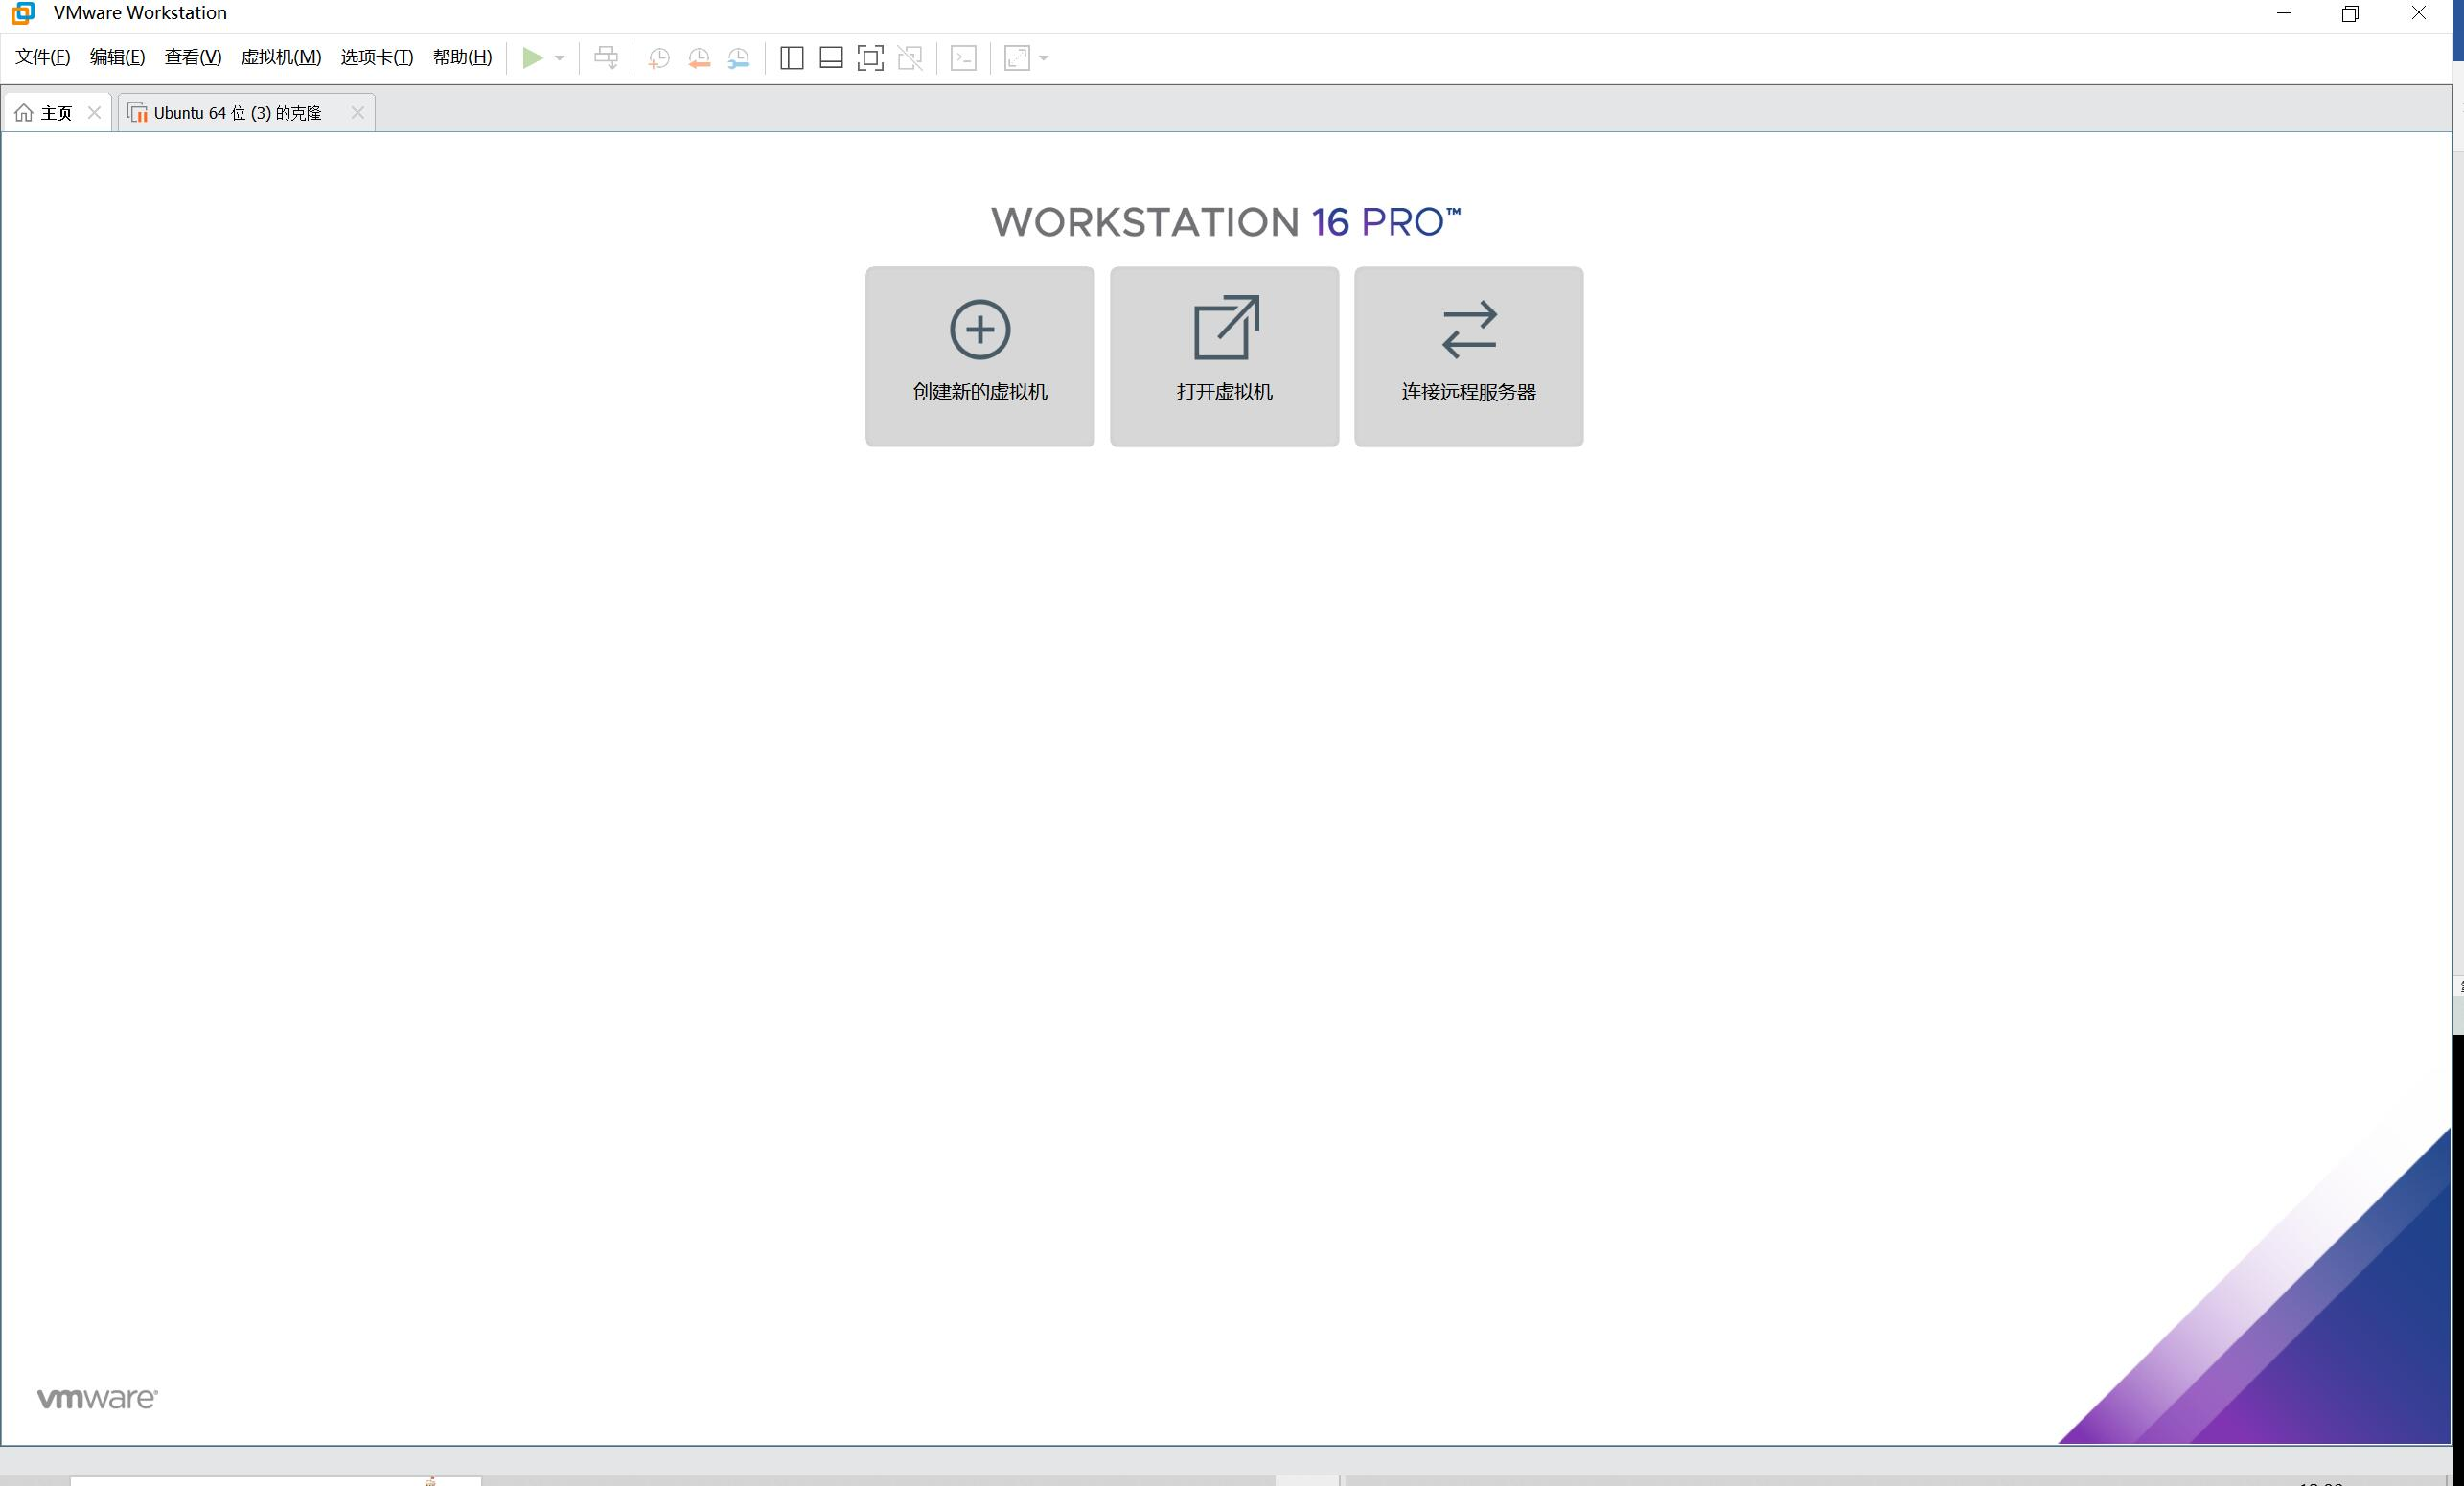
\includegraphics[width=0.8\textwidth]{figures/chapter2/2-1.jpg}
  \caption{VMware Workstation 16主界面}
  \label{fig:2 VMware Workstation 16主界面}
\end{figure}

\subsection{Ubuntu}

Ubuntu是基于Debian的桌面Linux操作系统,提供稳定和新颖的自由软件,有庞大的社区力量。如下图 2-2 所示为 Ubuntu 操作系统的截图。

\begin{figure}[H]
  \centering
  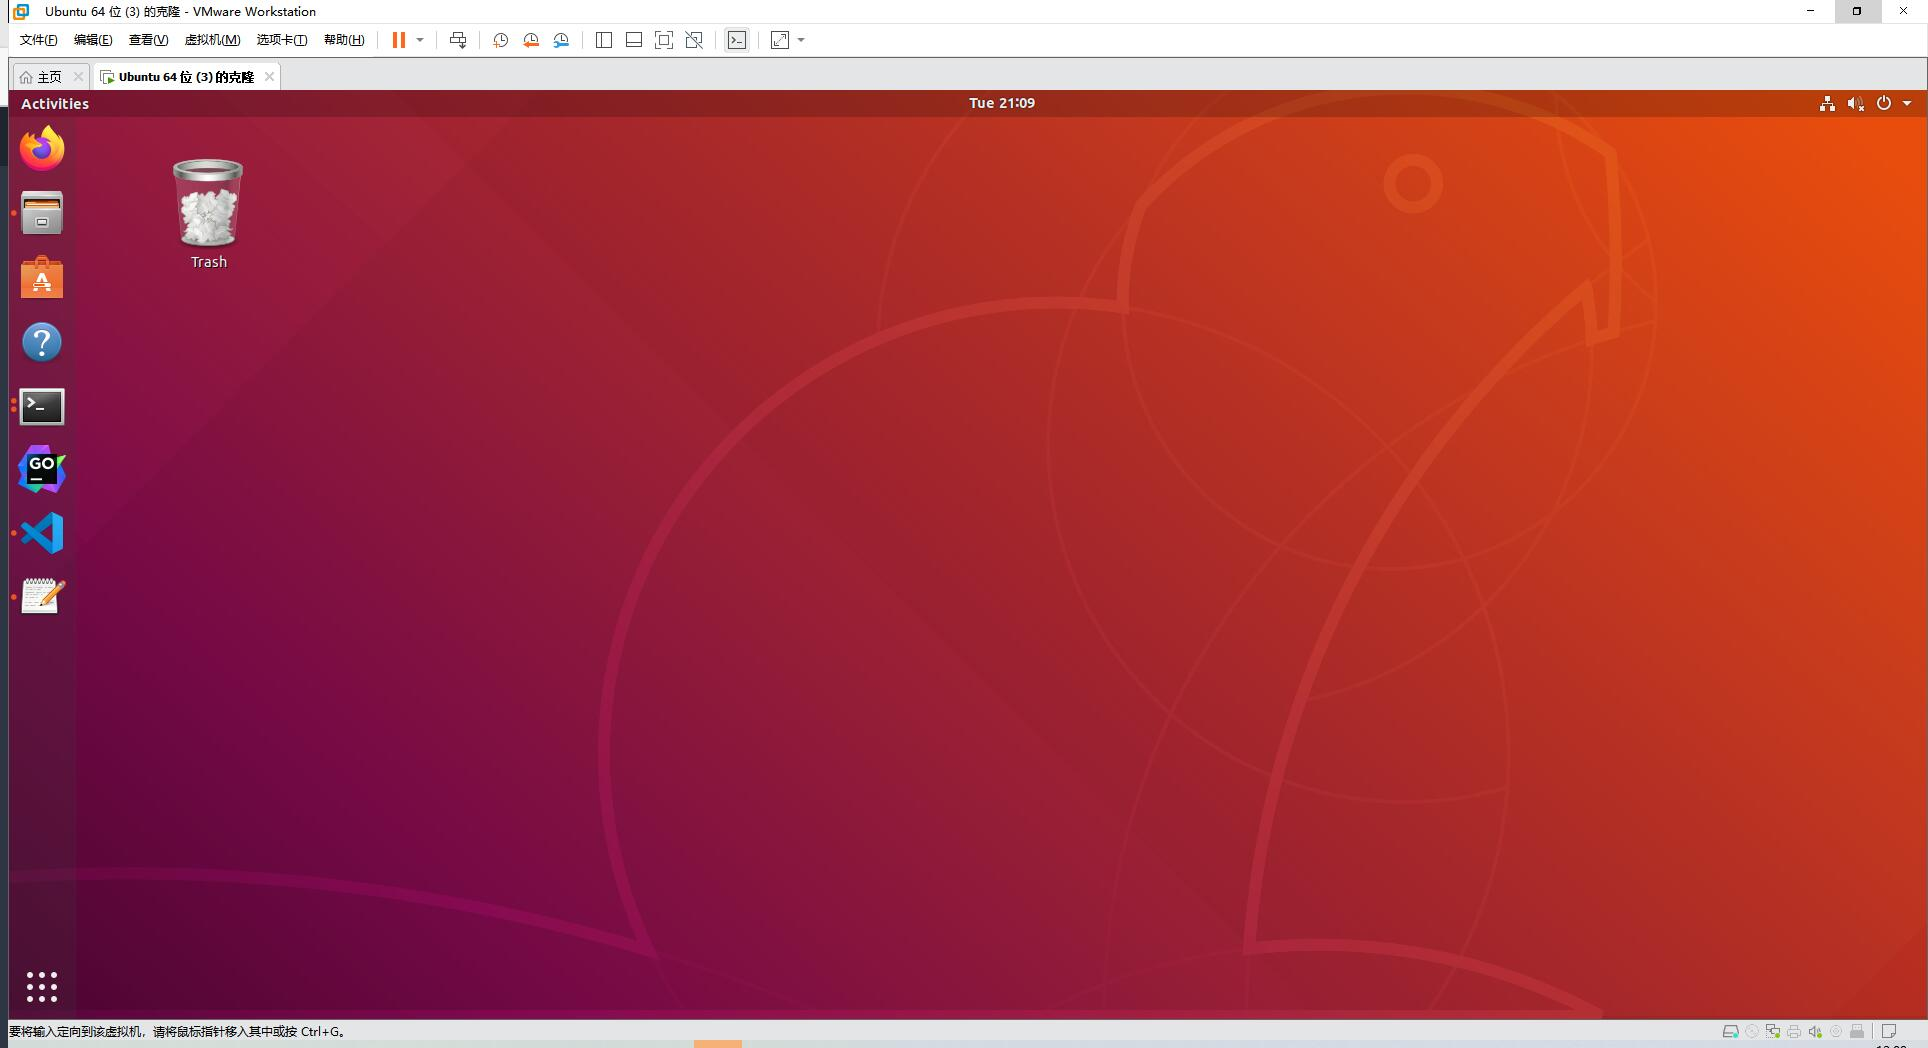
\includegraphics[width=0.8\textwidth]{figures/chapter2/2-2.jpg}
  \caption{Ubuntu 操作系统(虚拟机)主界面}
  \label{fig:2 Ubuntu 操作系统(虚拟机)主界面}
\end{figure}

\subsection{Bochs}

Bochs是一款开源的x86硬件平台模拟器,模拟整个PC平台,包括I/O设备、内存和BIOS。它能在多种平台上运行,并支持模拟多台PC。

\subsection{NASM、GCC 和 GNU MAKE}

Netwide Assembler(NASM)是x86架构的汇编与反汇编工具,支持多种二进制格式输出,适用于编写16位、32位和64位程序,以及创建引导加载程序等。遵循Intel风格汇编。


\section{调试过程及运行结果}

在安装完虚拟机和相应的 Linux 环境之后,为了能够对编写的源代码进行编译和仿真,还必须下载 Bochs。选择2.3.5版本。编译过程如下:

\begin{lstlisting}[language=bash]
  \tar vxzf bochs-2.3.5.tar.gz
  \cd bochs-2.3.5
  \./configure –enable-debbugger –enable-disasm 
  \make
  \sudo make install
\end{lstlisting}

如下图 2-3 所示为 Bochs 的运行界面。

\begin{figure}[H]
  \centering
  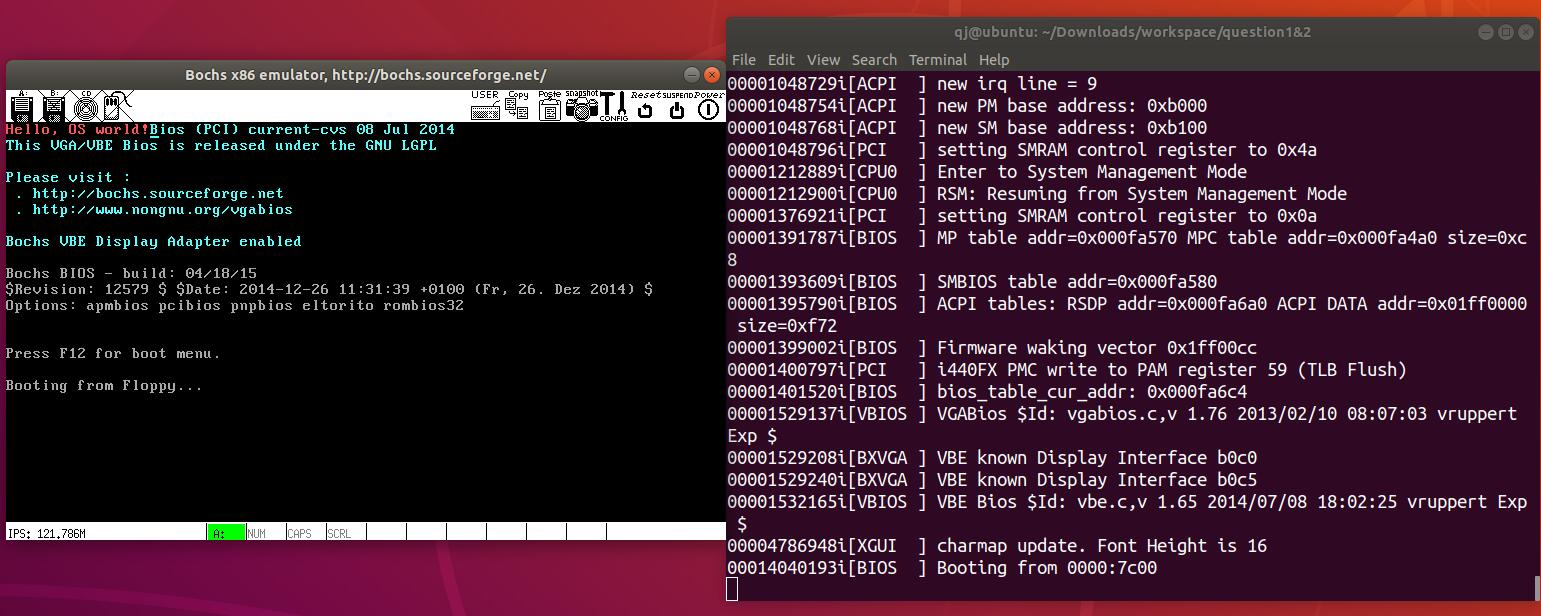
\includegraphics[width=0.8\textwidth]{figures/chapter2/2-3.jpg}
  \caption{Bochs运行界面}
  \label{fig:3}
\end{figure}

为了编译汇编语言,必须安装 NASM 程序,同时,还必须安装 GNU Make,用于自动化编译和链接。\par
在 Ubuntu 中已经预安装了 GCC,对于 GNU Make,可以通过以下的指令完成:
\begin{lstlisting}[language=bash]
  \sudo apt-get install build-essential nasm
\end{lstlisting}
从官网 https://www.nasm.us/下载NASM安装包,然后提取文件到指定文件夹,在文件夹下打开终端,依次输入下列指令:

\begin{lstlisting}[language=bash]
  \./configure
  \make
  \sudo make install
\end{lstlisting}

输入nasm -version指令来检验是否安装成功。

\section{实验总结}

搭建环境实验时,遇到了以下问题。报错:
00000000000p[ ] >>PANIC<< bochsrc:10: vgaromimage directive malformed.通过该报错信息,尝试
修改bochsrc与本地bochs组件路径对应:\par
\begin{enumerate}
    \item romimage: file=/usr/share/bochs/BIOS-bochs-latest
    \item vgaromimage: /usr/share/vgabios/vgabios.bin
    \item keyboard$\_$mapping:enabled=1,map=/usr/share/bochs/keymaps/x11-pc-us.map
\end{enumerate}\par
修改为:
\begin{enumerate}
    \item romimage:file=/home/qj/Downloads/workspace/bochs-2.6.8/bios/BIOS-bochs-latest
    \item vgaromimage:file=/home/qj/Downloads/workspace/bochs-2.6.8/bios/VGABIOS-lgpl-latest
    \item keyboard:keymap=/home/qj/Downloads/workspace/bochs-2.6.8/gui/keymaps/x11-pc-us.map
\end{enumerate}

即可解决问题。\par

总而言之,本章实验中出现了一些配置文件路径更改的问题,需要花费一些时间去查验。但我认为单纯解决问题还不够,应该了解问题出现的具体原因、解决方法以及解决方法的原理。因此,我去查阅了相关资料\cite{romimage},认识到 vgaromimage 指令用于指定 Bochs 模拟器使用的 VGA BIOS ROM 映像文件。VGA BIOS 用于控制 VGA 显示适配器的固件程序,它包含了一些基本的图形和显示功能。在 Bochs 模拟器中,通过设置 vgaromimage 指令,可以指定要加载的 VGA BIOS ROM 映像文件的路径和文件名。Bochs 在启动时会读取该指令并加载相应的 VGA BIOS ROM 映像文件。而 VGA BIOS ROM 映像文件通常是一个二进制文件,其中包含了 VGA BIOS 的固件代码。这些代码实现了 VGA 显示适配器的初始化、显示模式设置、图形绘制和显示输出等功能。

\chapter{动手写一个最小的“操作系统”}
 
\section{实验内容}

通过编译一段最基本的 asm 代码来初次体验操作系统的设计以及了解NASM 编译的使用方法、dd 命令写入磁盘的方法以及 Bochs 的使用方法。

\section{代码分析}

\subsection{核心数据结构}
常量 BootMessage:	db "Hello, OS world!"

\subsection{关键代码分析}

\begin{lstlisting}[language = C]
org 07c00h	; 告诉编译器程序加载到 7c00 处
#使 ds 和 es 两个寄存器指向与 cs 相同的段
mov ax, cs
mov ds, ax
mov es, ax
call	DispStr	; 调用显示字符串例程
jmp $	; 无限循环
DispStr:
mov ax, BootMessage
mov bp, ax	; ES:BP = 串地址
mov cx, 16	; CX = 串长度
mov ax, 01301h	; AH = 13, AL = 01h

mov bx,	000ch		;	页号为 0(BH = 0) 黑底红字(BL = 0Ch,高亮)
mov dl,	0			
int 10h		;	10h	号中断
ret				
BootMessage:	db	"Hello, OS world!"
times 510-($-$$)	db	0  ; 填充剩下的空间,使生成的二进制代码恰好为512 字节		
dw	0xaa55		; 结束标志
\end{lstlisting}
值得注意的是,未被方括号括起来的变量名被看作是地址,如果不加方括号时出现数字,则视作 offset;\$表示当前行被汇编后的地址,\$\$表示一个节的开始处被汇编之后的地址。

\section{调试过程及运行结果}

想要进行操作系统的调试,首先必须创建一个软盘映像,在 terminal 中输入 bximage 即可打开相应的界面。根据引导界面,依次输入 1->fd->回车->回车,即可生成一个名为 a.img的软盘映像,如下图 3-1 所示。
\begin{figure}[H]
  \centering
  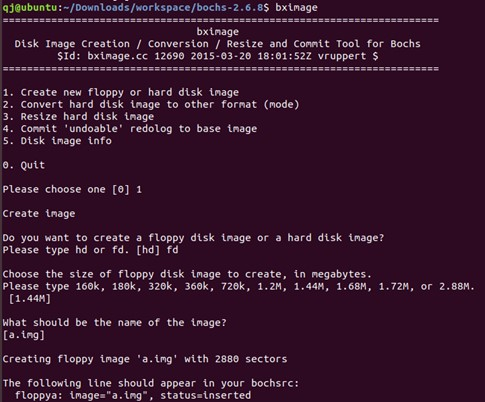
\includegraphics[width=0.7\textwidth]{figures/chapter3/3-1.jpg}
  \caption{bximage操作界面}
  \label{fig:1}
\end{figure}

创建完软盘映像后,需要编译源代码,输入以下命令即可完成编译。
\begin{lstlisting}[language = bash]
  \nasm boot.asm -o boot.bin
\end{lstlisting}

完成编译之后,我们需要使用软盘绝对扇区读写工具将这个文件写到一张空白软盘的第一个扇区,输入以下代码即可完成读入。
\begin{lstlisting}[language = bash]
  \dd if=boot.bin of=a.img bs=512 count=1 conv=notrunc
\end{lstlisting}
一切准备就绪之后,需编写 Bochs 的配置文件 bochsrc.disk,即告诉 Bochs 对虚拟机中内存,硬盘映像和软盘映像等的配置信息:\par
\# what disk images will be used\par
floppya: 1$\_$44=a.img, status=inserted\par
\# choose the boot disk.\par
boot: a\par

上述步骤完成之后,一切准备就绪,正式进行调试,输入命令:
\begin{lstlisting}[language = bash]
  \bochs -f bochsrc
\end{lstlisting}
按下回车键,再选择6,会出现如下图 3-2 所示的界面。
\begin{figure}[H]
  \centering
  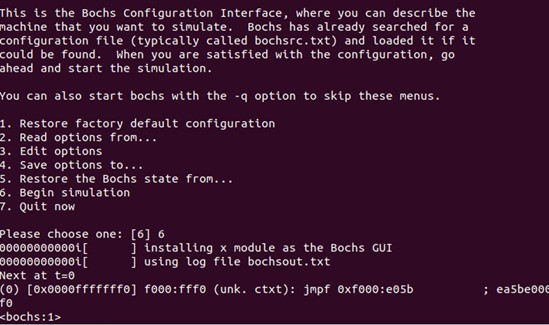
\includegraphics[width=0.7\textwidth]{figures/chapter3/3-2.jpg}
  \caption{调试过程}
  \label{fig:2}
\end{figure}

输入 c,即会进入 bochs 页面,这时,屏幕的左上角会出现一行红色的“Hello, OS world!”,即代表调试成功。调试结果如下图 3-3 所示。
\begin{figure}[H]
  \centering
  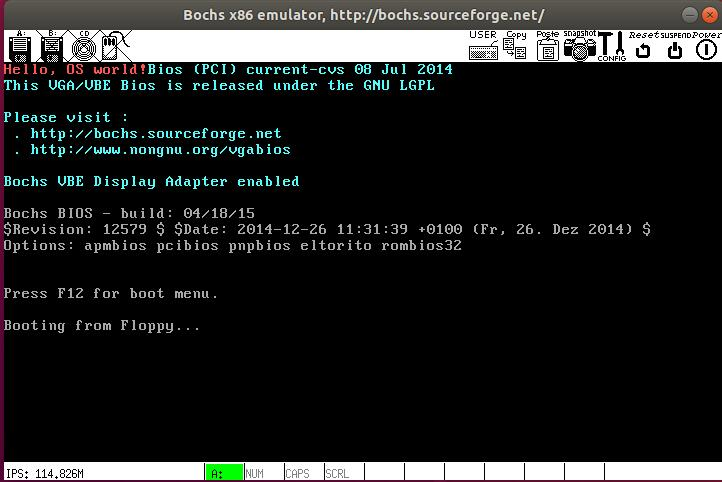
\includegraphics[width=0.8\textwidth]{figures/chapter3/3-3.jpg}
  \caption{调试结果}
  \label{fig:3}
\end{figure}

\section{实验总结}
在本实验中,我们编写了一个最简单的“操作系统”,并且使用 Bochs 软件进行仿真。但是事实上,我们编写的程序只是一个最简单的引导扇区,之所以可以称之为最简单的操作系统,是因为它可以直接在裸机上运行。计算机电源打开时,首先会加电自检,然后寻找启动盘,如果是选择从软盘启动,计算机就会检查软盘的 0 面 0 磁道 1 扇区,如果发现它以 0xAA55 结束,那么 BIOS 就会认为它是一个引导扇区。\par
当然,一个正确的引导扇区除了以 0xAA55结束之外,还应该包含一段少于 512 字节的执行码。而一旦 BIOS 发现了引导扇区,就会将这 512 字节的内容装载到内存地址 0000:7c00 处,然后跳转到 0000:7c00 处,将控制权彻底交给这段引导代码。至此为止,计算机不再由 BIOS中固有的程序来控制,而是变为由操作系统的一部分来控制。我们编写的代码中第一行就是将程序加载到 0x7c00 处,第十八行是让代码以 0xAA55 结束,因而可以作为一个独立的引导扇区运行。\par
总而言之,第二个实验的任务是一个最小的操作系统,也就是在虚拟机上运行 Helloworld。首先是 nasm 的编译,编译.asm 变为.bin,可以制作引导扇区,编译变为.com,可以调试。之后是 dd 命令写入磁盘,主要是 dd if=boot.bin of=/dev/fd0 bs=512 count=1 conv=notrunc(防止截断)。软盘读写工具将文件写到空白软盘的第一个扇区,然后让 ds 和es 两个段寄存器指向与cs 相同的段,调用子程序显示字符串,然后无限循环。最后是 bochs 的用法,用 bximage 命令创建一个空白映像文件,再使用 dd 命令将.bin 文件写入,撰写一个 bochsrc 文件,指定从软盘启动,并且使用.bin 文件。启动后使用以下命令进行调试:b 设置断点, c 继续执行, dump$\_$cpu查看寄存器, x 查看内存, n 运行下一条指令。实验二思维导图如下图3-4所示:
\begin{figure}[H]
  \centering
  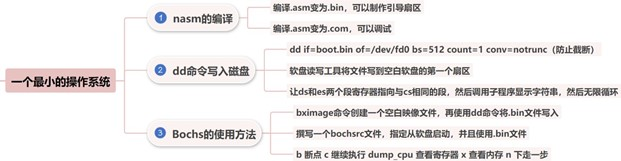
\includegraphics[width=0.8\textwidth]{figures/chapter3/3-4.jpg}
  \caption{实验二思维导图}
  \label{fig:3}
\end{figure}

 \vfill
\chapter{实现保护模式}\label{cha:latex-brief-intro}
为了使实验报告清晰简洁,后续实验均省略了部分具体代码实现部分,仅重点说明主要数据和代码结构,以体现设计的核心思想。

\section{实验内容}
认识保护模式,实现从实模式到保护模式的转换,GDT 描述符;实现实模式大于 1MB 内存的寻址能力,并接着上一次实验,从保护模式返回到实模式,重新设置各个段寄存器的值;LDT 描述符;学会使用挂载指令和运行程序。

\section{代码分析}

\subsection{核心数据结构}

\begin{table}[H]
\begin{center}
\caption{[SECTION .gdt]段 gdt数据段}
\begin{tabular}{|c|ll|}
\hline
\multirow{3}{*}{数组 GDT} & \multicolumn{2}{l|}{LABEL\_GDT 空描述符}                 \\ \cline{2-3} 
                        & \multicolumn{2}{l|}{LABEL\_DESC\_CODE32 非一致代码段32描述符} \\ \cline{2-3} 
                        & \multicolumn{2}{l|}{LABEL\_DESC\_VIDEO 显存首地址}        \\ \hline
\multirow{2}{*}{变量}     & \multicolumn{2}{l|}{Gdtlen 表示GDT的长度}                 \\ \cline{2-3} 
                        & \multicolumn{2}{l|}{GdtPtr dw为GDT界限 dd为GDT基址}        \\ \hline
\multirow{2}{*}{选择子}    & \multicolumn{2}{l|}{SelectorCode32 非一致代码段32选择子}      \\ \cline{2-3} 
                        & \multicolumn{2}{l|}{SelectorVideo 视频段选择子}            \\ \hline
\end{tabular}
\end{center}
\end{table}
如表 4-1 所示,该部分对应“认识保护模式,实现从实模式到保护模式的转换,认识 GDT 描述符,并进入保护模式”的数据结构。

\begin{table}[H]
\begin{center}
    \caption{[SECTION .gdt]段 gdt数据段}
\begin{tabular}{|c|l|l|}
\hline
\multirow{8}{*}{数组 GDT}                 & LABEL\_GDT          & 空描述符                       \\ \cline{2-3} 
                                        & LABEL\_DESC\_NORMAL & Normal 描述符                 \\ \cline{2-3} 
                                        & LABEL\_DESC\_CODE32 & 非一致代码段 32 描述符              \\ \cline{2-3} 
                                        & LABEL\_DESC\_CODE16 & 非一致代码段 16 描述符              \\ \cline{2-3} 
                                        & LABEL\_DESC\_DATA   & 数据段描述符                     \\ \cline{2-3} 
                                        & LABEL\_DESC\_STACK  & 32 位堆栈段描述符                 \\ \cline{2-3} 
                                        & LABEL\_DESC\_TEST   & 测试段描述符                     \\ \cline{2-3} 
                                        & LABEL\_DESC\_VIDEO  & 显存描述符                      \\ \hline
\multirow{2}{*}{变量}                     & Gdtlen              & 表示 GDT 的长度                 \\ \cline{2-3} 
                                        & GdtPtr              & \begin{tabular}
                                                                [c]{@{}l@{}}前两个字节为GDT界限\\ 
                                                                后四个字节为GDT基址\end{tabular} \\ \hline
\multirow{2}{*}{选择子}                    & SelectorNormal      & Normal 选择子                 \\ \cline{2-3} 
                                        & SelectorCode32      & 非一致代码段 32 选择子              \\ \hline
\multicolumn{1}{|l|}{\multirow{5}{*}{}} & SelectorCode16      & 非一致代码段 16 选择子              \\ \cline{2-3} 
\multicolumn{1}{|l|}{}                  & SelectorData        & 数据段选择子                     \\ \cline{2-3} 
\multicolumn{1}{|l|}{}                  & SelectorStack       & 堆栈段选择子                     \\ \cline{2-3} 
\multicolumn{1}{|l|}{}                  & SelectorTest        & 测试段选择子                     \\ \cline{2-3} 
\multicolumn{1}{|l|}{}                  & SelectorVideo       & 视频段选择子                     \\ \hline
\end{tabular}
\end{center}
\end{table}

\begin{table}[H]
\begin{center}
\caption{[SECTION .data1] 数据段}
\begin{tabular}{|c|l|l|}
\hline
\multirow{6}{*}{常量} & SPValueInRealMode & 字符串                                                                     \\ \cline{2-3} 
                    & PMMessage         & 在保护模式中显示的信息"In Protect Mode now. \textasciicircum{}-\textasciicircum{}" \\ \cline{2-3} 
                    & OffsetPMMessage   & PMMessage 段偏移                                                           \\ \cline{2-3} 
                    & StrTest           & “ABCDEFGHIJKLMNOPQRSTUVWXYZ”                                            \\ \cline{2-3} 
                    & OffsetStrTest     & StrTest 段偏移                                                             \\ \cline{2-3} 
                    & DataLen           & 表示数据段的长度                                                                \\ \hline
\end{tabular}
\end{center}
\end{table}

\begin{table}[H]
\begin{center}
\caption{[SECTION .gs] 全局堆栈段}
\begin{tabular}{|c|l|l|}
\hline
常量 & TopOfStack & 栈顶指针 \\ \hline
\end{tabular}
\end{center}
\end{table}

如表 4-2、4-3、4-4 所示,该部分对应“实现实模式大于 1MB 内存的寻址,并接着上一次实验,在 DOS 模式下从保护模式返回到实模式,重新设置各个段寄存器的值”的数据结构。

\begin{table}[H]
\begin{center}
\caption{[SECTION .ldt]段 LDT数据段}
\begin{tabular}{|c|l|l|}
\hline
\multirow{3}{*}{LDT 数组} & LABEL\_LDT\_DESC\_CODEA & LDT 描述符    \\ \cline{2-3} 
                        & LDTLen                  & 表示 LDT 的长度 \\ \cline{2-3} 
                        & SelectorLDTCodeA        & LDT 选择子    \\ \hline
\end{tabular}
\end{center}
\end{table}

如表 4-2、4-3、4-4、4-5 所示,该部分对应“了解 LDT 描述符;学会使用挂载指令将文件挂载在临时目录和并运行程序”的数据结构。

\subsection{关键代码段分析}
\begin{enumerate}
    \item \texttt{[SECTION .s16][BITS 16]} --- 代码段:从实模式跳到保护模式
    \begin{itemize}
        \item 初始化 32 位代码段描述符:将 \texttt{[SECTION .S32]} 段的物理地址分三部分赋给空白描述符 \texttt{DESC\_CODE32}
        \item 为加载 \texttt{GDTR} 做准备:将 \texttt{GDT} 的物理地址填充到 \texttt{GdtPtr} 中
        \item 加载 \texttt{GDTR}:将 \texttt{GdtPtr} 加载到寄存器 \texttt{gdtr} 中
        \item 关中断
        \item 打开 \texttt{A20} 地址线:通过操作端口 \texttt{92h}
        \item 准备切换到保护模式:把寄存器 \texttt{cr0} 的第 0 位置为 1
        \item 进入保护模式:\texttt{Jump}
    \end{itemize}
    
    \item \texttt{[SECTION .s32][BITS 32]} --- 32 位代码段,由实模式跳入。将视频段选择子 \texttt{SelectorVideo} 的地址赋给 \texttt{gs}
    \begin{itemize}
        \item 设置输出位置为屏幕 11 行 79 列
        \item 设置输出为黑底红字
        \item 往显存中 \texttt{edi} 偏移处写入 \texttt{P}
        \item 无限循环
    \end{itemize}
    
    \item 从保护模式跳回到实模式
    \begin{itemize}
        \item 程序重设各个段寄存器值,使 \texttt{ds}、\texttt{es}、\texttt{ss} 指向 \texttt{as}
        \item 恢复 \texttt{sp} 的值
        \item 关闭 \texttt{A20}
        \item 打开中断
        \item 回到 DOS
    \end{itemize}
    
    \item \texttt{[SECTION .s32]} --- 32 位代码段,由实模式跳入。初始化 \texttt{ds}、\texttt{es}、\texttt{gs}、\texttt{ss}:
    \begin{itemize}
        \item \texttt{ds} 指向数据段
        \item \texttt{es} 指向新增的 5MB 的内存段
        \item \texttt{gs} 指向显存
        \item \texttt{ss} 指向测试段
        \item 显示一个字符串
        \item 调用读内存函数 \texttt{TestRead}
        \item 调用写函数 \texttt{TestWrite}
        \item 调用函数 \texttt{TestRead}
        \item 跳转到 \texttt{[SECTION .s16code]} 代码段的 \texttt{TestRead} 函数
    \end{itemize}
    
    \item \texttt{[SECTION .s16code]} --- 16 位代码段,由 32 位代码段跳入,跳出后到实模式
    \begin{itemize}
        \item 把选择子 \texttt{SelectorNormal} 加载到 \texttt{ds}、\texttt{es}、\texttt{ss}
        \item 清 \texttt{cr0} 的 \texttt{PE} 位,跳回实模式
        \item 跳转到 \texttt{LABEL\_REAL\_ENTRY} 即段 \texttt{[SECTION .s16]} 里
    \end{itemize}
\end{enumerate}


\section{调试过程及运行结果}

在之前的实验过程中,我们将文件写到了引导扇区运行,但引导扇区只有 512 个字节。空间有限。为使程序扩大,可以选择先借用其他操作系统的引导扇区,我们借用 DOS 操作系统,将程序编译成 COM 文件,然后用 DOS 来执行它。第一步需要到 Bochs 官方网站下载一个 FreeDos,解压后将其中的 a.img 复制到我们的工作目录中,并改名为 freedos.img。紧接着,我们需要使用 bximage 生成一个软盘映像,取名为 pm.img。再其次,我们需要修改我们的 bochsrc与上述img文件对应。最后,直接启动 Bochs 开始调试,即可进入 FreeDos 界面,输入 format b 的指令以便格式化 freedos 的 B:盘。格式化及格式化结果如下图 4-1 所示。
\begin{figure}[H]
  \centering
  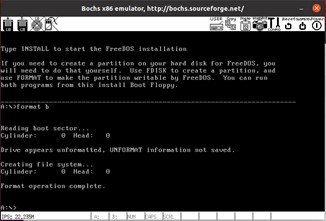
\includegraphics[width=0.8\textwidth]{figures/chapter4/4-1.jpg}
  \caption{freedos格式化B盘示意图}
  \label{fig:1}
\end{figure}

格式化完成后,将上述代码第 8 行中的 07c00h 改为 0100h,并重新编译为 com 文件:
\begin{lstlisting}[language = bash]
  \nasm pmtest1.asm -o pmtest1.com
\end{lstlisting}
紧接着,我们需要输入以下三条指令,将 pmtest1.com 复制到虚拟软盘pm.img 中,所需要的指令如下:
\begin{lstlisting}[language = bash]
  \sudo mount -o loop pmimg /mnt/floppy
  \sudo cp pmtest1.com /mnt/floppy
  \sudo umount /mnt/floppy
\end{lstlisting}
此时若出现挂载点不存在的错误,输入以下指令即可解决:
\begin{lstlisting}
  \sudo mkdir /mnt/floppy
\end{lstlisting}
接下来我们需要重新回到 FreeDos 中(即原先打开的 Bochs 虚拟机),并且输入如下命令:
\begin{lstlisting}[language = bash]
  \b:\pmtest1.com
\end{lstlisting}
pmtest1.com 成功运行。可以注意到,一个红色的字母“P”出现在了屏幕的右侧的中部,这代表调试成功,程序已经进入了保护模式。调试结果如下图 4-2 所示。
\begin{figure}[H]
  \centering
  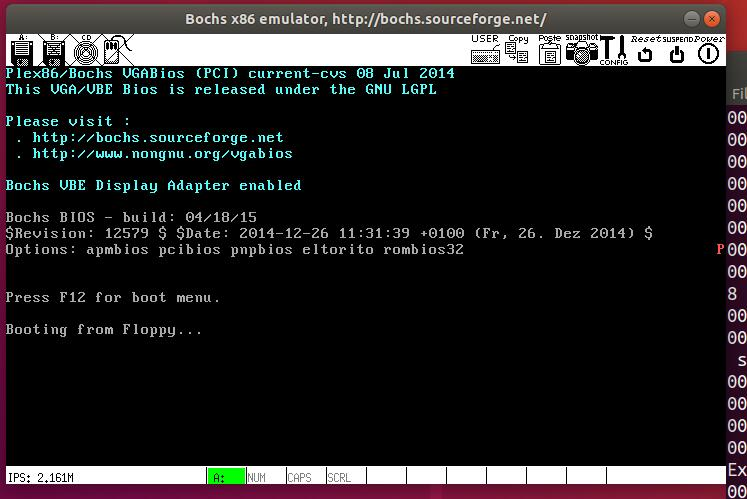
\includegraphics[width=0.8\textwidth]{figures/chapter4/4-2.jpg}
  \caption{pmtest1.com 调试结果}
  \label{fig:2}
\end{figure}

下一步以同样方式运行pmtest2.com。调试结果如下图 4-3 所示,可以看到,程序打印出了两行数字,第一行全部是 0,说明开始内存 5MB 处都是 0,而下一行已经变成了 41、42、43...,说明写操作成功(十六进制的 41、42、43...48 正是 A、B、C...H)。同时可以看到,程序执行结束后没有进入死循环,而是重新出现了 DOS 提示符,这说明我们已经重新到了实模式下的 DOS。
\begin{figure}[H]
  \centering
  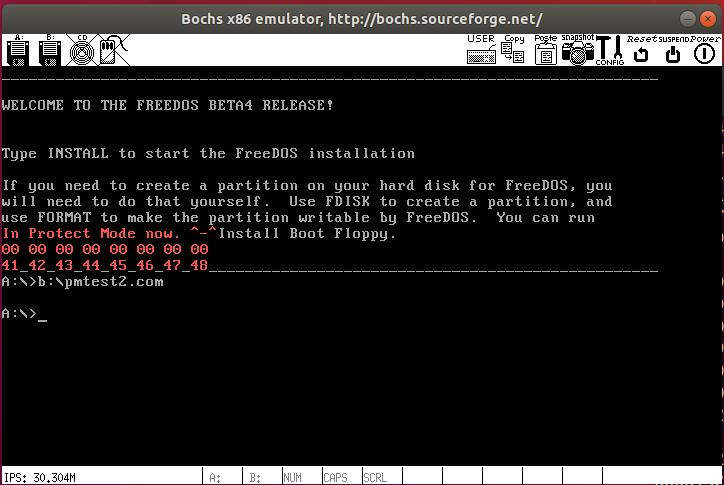
\includegraphics[width=0.8\textwidth]{figures/chapter4/4-3.jpg}
  \caption{pmtest2.com运行结果图}
  \label{fig:3}
\end{figure}

最后再以同样方式运行pmtest3.com。此处 LDT 中的代码段只是打印一个字符 L,因此,在[SECTION .s32]中打印完“In Protect Mode Now.”这个字符串之后,一个红色的字符 L 将会出现。可以看到在下图 4-4 中,的确出现了“In Protect Mode Now.”字符串和一个红色的 L。
\begin{figure}[H]
  \centering
  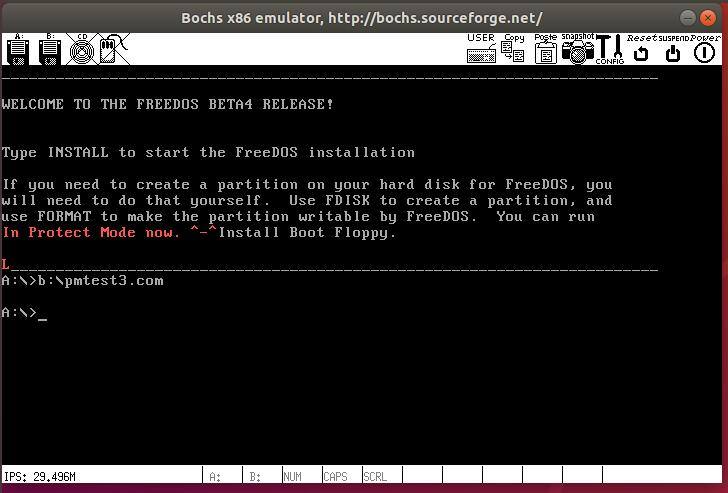
\includegraphics[width=0.8\textwidth]{figures/chapter4/4-4.jpg}
  \caption{pmtest3.com运行结果图}
  \label{fig:4}
\end{figure}

\section{实验总结}

CPU 通常情况下有两种工作模式:实模式和保护模式。打开计算机时CPU默认工作在实模式下,现在需要让其进入保护模式,发挥其寻址能力,并为 32 位系统提供硬件保障。本实验中,在 pm.inc 文件中定义了全局描述表 GDT,定义了相应的段描述符,并且通过 pmtest1.com 由实模式进入保护模式,最后在保护模式中在屏幕右边中央打印了一个红色的“P”,代表实验成功。在调试过程中,我发现只需要将b盘格式化一次,后面就不需要再格式化了。\par
接着,系统成功进入保护模式,打印了一个红色的 P,在本实验中,我们重新建立了一个以 5MB 为基址的段,随后先读出开始处 8 字节的内容,然后写入一个字符串,再从中读出 8 字节。如果读写成功,两次读出的内容不同,而且第二次读出的内容应该前面写进的字符串。然后返回实模式,我们加载了一个合适的描述符选择有关段寄存器,以使对应的段描述符和高速缓存寄存器中含有合适的段界限和属性。而且,我们不能从 32 位代码段返回实模式,只能从 16 位代码段中返回,这是因为无法实现从 32位代码段返回时 cs 高速缓存寄存器中的属性符合实模式的要求(实模式不能改变段属性)。\par
最后,我了解并学习了描述符表LDT,LDT 与 GDT 类似,但它的段选择子的 T1 位必须为 1。类似地,在运用它时,必须先用 lldt 指令加载 ldtr,而 ldtr 的操作数是 GDT 中用来描述 LDT 的段描述符。\par
为了补充相关理论知识,我去查阅相关资料\cite{80286与保护模式}。结合上述实验,我认识到保护模式是 x86 处理器中的一种特殊的操作模式,它与硬件紧密结合,提供了更高级的内存保护和多任务支持。通过将内存划分为多个段并为每个段设置不同的访问权限和保护级别,从而可以防止程序越界访问内存和修改其他程序的数据,提高系统的稳定性和安全性。同时,在保护模式下的操作系统可以实现多任务,每个程序拥有独立的内存空间和代码段,通过任务切换来实现并发执行。结合并发这一点,LDT的引入便显得十分自然,GDT 是全局描述符表,存储了系统中所有进程和任务的段描述符;LDT 是局部描述符表,用于存储特定任务或进程的私有段描述符。通过使用 GDT 和 LDT,操作系统可以对不同任务或进程的内存访问权限进行细粒度控制,提高系统的安全性和灵活性,从而更好地实现并发。

\chapter{切换到保护模式}\label{cha:latex-brief-intro}

\section{实验内容}
引导扇区突破 512 个字节的限制,将工作分给 loader;加载 loader 进入内存并运行;将控制权交给 loader。

\section{代码分析}

\subsection{核心数据结构}

% Please add the following required packages to your document preamble:
% \usepackage{multirow}
\begin{table}[htbp]
\begin{center}
\caption{boot.asm的主要数据结构}
\begin{tabular}{|c|l|l|}
\hline
\multirow{19}{*}{\begin{tabular}[c]{@{}c@{}}FAT12\\    \\ 格式\end{tabular}} & BS\_OEMName     & OEM String, 必须 8 个字节        \\ \cline{2-3} 
                                                                           & BPB\_BytsPerSec & 每扇区字节数:512                  \\ \cline{2-3} 
                                                                           & BPB\_SecPerClus & 每簇扇区数:1                     \\ \cline{2-3} 
                                                                           & BPB\_RsvdSecCnt & Boot 记录占用扇区数:1              \\ \cline{2-3} 
                                                                           & BPB\_NumFATs    & FAT 表数码:2                   \\ \cline{2-3} 
                                                                           & BPB\_RootEntCnt & 根目录文件数最大值:224               \\ \cline{2-3} 
                                                                           & BPB\_TotSec16   & 逻辑扇区总数:2880                 \\ \cline{2-3} 
                                                                           & BPB\_Media      & 媒体描述符:0xF0                  \\ \cline{2-3} 
                                                                           & BPB\_FATSz16    & 每 FAT 扇区数:9                 \\ \cline{2-3} 
                                                                           & BPB\_SecPerTrk  & 每磁道扇区数:18                   \\ \cline{2-3} 
                                                                           & BPB\_NumHeads   & 磁头数(面数:2                    \\ \cline{2-3} 
                                                                           & BPB\_HiddSec    & 隐藏扇区数:0                     \\ \cline{2-3} 
                                                                           & BPB\_TotSec32   & 这个值记录扇区数:0                  \\ \cline{2-3} 
                                                                           & BS\_DrvNum      & 中断 13 的驱动器号:0               \\ \cline{2-3} 
                                                                           & BS\_Reserved1   & 未使用:0                       \\ \cline{2-3} 
                                                                           & BS\_BootSig     & 扩展引导标记 (29h)                \\ \cline{2-3} 
                                                                           & BS\_VolID       & 卷序列号                        \\ \cline{2-3} 
                                                                           & BS\_VolLab      & 卷标, 必须 11 个字节:'OrangeS0.02' \\ \cline{2-3} 
                                                                           & BS\_FileSysType & 文件系统类型, 必须 8 个字节:'FAT12’    \\ \hline
常量                                                                         & BootMessage     & "Hello, OS world!"          \\ \hline
\end{tabular}
\end{center}
\end{table}
如下表 5-1 所示,此处对应的是“引导扇区加上 BPB 等头信息,可以被 DOS 识别,引导扇区突破 512 个字节的限制,将工作分给 loader”部分的主要数据结构。


% Please add the following required packages to your document preamble:
% \usepackage{multirow}
\begin{table}[H]
\begin{center}
\caption{对boot.asm增添的部分}
\begin{tabular}{|cl|l|l|}
\hline
\multicolumn{2}{|c|}{\multirow{3}{*}{变量}}  & wRootDirSizeForLoop     & Root Directory 占用的扇区数      \\ \cline{3-4} 
\multicolumn{2}{|c|}{}                     & wSectorNo               & 要读取的扇区号                    \\ \cline{3-4} 
\multicolumn{2}{|c|}{}                     & bOdd                    & 奇数还是偶数                     \\ \hline
\multicolumn{2}{|c|}{\multirow{4}{*}{字符串}} & LoaderFileName          & LOADER.BIN 文件名             \\ \cline{3-4} 
\multicolumn{2}{|c|}{}                     & BootMessage             & "Booting"                  \\ \cline{3-4} 
\multicolumn{2}{|c|}{}                     & Message1                & "Ready."                   \\ \cline{3-4} 
\multicolumn{2}{|c|}{}                     & Message2                & "No LOADER"                \\ \hline
\multicolumn{2}{|c|}{\multirow{5}{*}{宏}}   & BaseOfStack             & 调试状态下堆栈基地址                 \\ \cline{3-4} 
\multicolumn{2}{|c|}{}                     & BaseOfLoader            & LOADER.BIN 被加载到的位置----段地址  \\ \cline{3-4} 
\multicolumn{2}{|c|}{}                     & OffsetOfLoader          & LOADER.BIN 被加载到的位置----偏移地址 \\ \cline{3-4} 
\multicolumn{2}{|c|}{}                     & RootDirSectors          & 根目录占用空间                    \\ \cline{3-4} 
\multicolumn{2}{|c|}{}                     & SectorNoOfRootDirectory & Root Directory 的第一个扇区号     \\ \hline
\end{tabular}
\end{center}
\end{table}
如表 5-2 所示,此处对应的是“加载 loader 进入内存并运行”部分在boot.asm基础上增添的主要数据结构。

\begin{table}[H]
\begin{center}
\caption{对boot.asm再次增添的部分}
\begin{tabular}{|c|l|l|}
\hline
\multirow{2}{*}{宏} & SectorNoOfFAT1 & FAT1 的第一个扇区号=BPB\_RsvdSecCnt                                                                            \\ \cline{2-3} 
                   & DeltaSectorNo  & \begin{tabular}[c]{@{}l@{}}DeltaSectorNo = BPB\_RsvdSecCnt \\ + (BPB\_NumFATs * FATSz) - 2\end{tabular} \\ \hline
\end{tabular}
\end{center}
\end{table}

如表 5-3 所示,此处对应的是“将控制权交给 loader”部分在上述boot.asm基础上再次增添的主要数据结构。


\subsection{关键代码分析}
\begin{enumerate}
    \item 使 \texttt{ds}、\texttt{es}、\texttt{ss} 三个段寄存器指向与 \texttt{cs} 相同的段,令栈指针 \texttt{sp} 指向栈底。清屏并显示字符串 \texttt{Booting}.
    
    \item 在 A 盘的根目录寻找 \texttt{LOADER.BIN}:遍历根目录取所有的扇区,将每一个扇区加载到内存,从中寻找文件名为 \texttt{Loader.bin} 的条目。每读一个扇区就在 "Booting " 后面打一个点。正式跳转到已加载到内存中的 \texttt{LOADER.BIN} 的开始处后显示字符串“Ready”,开始执行 \texttt{LOADER.BIN} 的代码。
    
    \item \texttt{ReadSector} 函数:从第 \texttt{ax} 个 Sector 开始,将 \texttt{cl} 个 Sector 读入 \texttt{es:bx} 中。
    
    \item \texttt{GetFATEntry} 函数:找到序号为 \texttt{ax} 的 Sector 在 FAT 中的条目,结果放在 \texttt{ax} 中。需要注意的是,在中间需要读 FAT 的扇区到 \texttt{es:bx} 处,所以函数一开始就保存了 \texttt{es} 和 \texttt{bx}。
    
    \item \texttt{Loader.asm}:
    令 \texttt{gs} 指向 \texttt{0B8h00h} 处,设置黑底白字。
    设置 \texttt{AL}='L'。
    在 \texttt{gs} 偏移处(屏幕第 0 行 39 列)写入 \texttt{L}。
\end{enumerate}


\section{调试过程及运行结果}

调试方法与上一个实验类似,不作重复阐述。调试结果如下图 5-1 所示。
\begin{figure}[H]
  \centering
  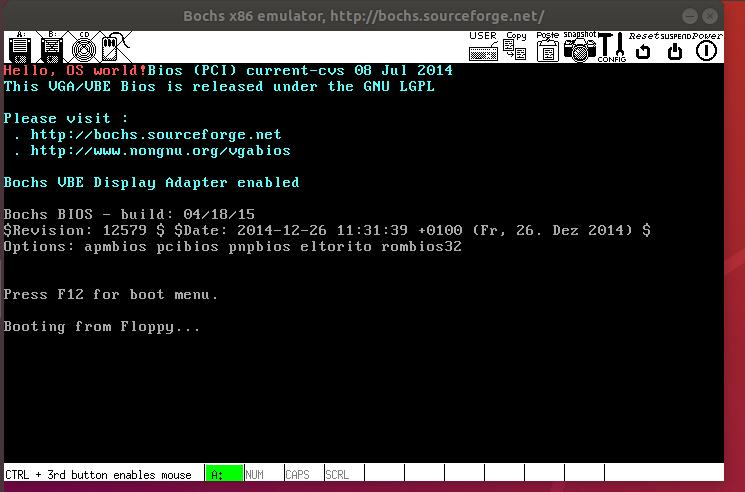
\includegraphics[width=0.8\textwidth]{figures/chapter5/5-1.jpg}
  \caption{引导扇区被DOS识别}
  \label{fig:1}
\end{figure}

这时我们已经为我们的引导扇区加入了 BPB 等头信息,使其可以被DOS识别。接着我们根据实验要求修改boot.asm,使其寻找loader.bin文件。由于我们仅仅是找到Loader.bin就停在那里,这时我们应该使用 Bochs 的调试功能。调试命令如下:
\begin{lstlisting}[language = bash]
  \b ox7c00
  \c
  \n
  \u /45
  \b 0x7cb4
  \c
  \x /32xb es:di -16
  \sreg
  \r
\end{lstlisting}
调试过程如下图 5-2、5-3、5-4 所示:

\begin{figure}[H]
  \centering
  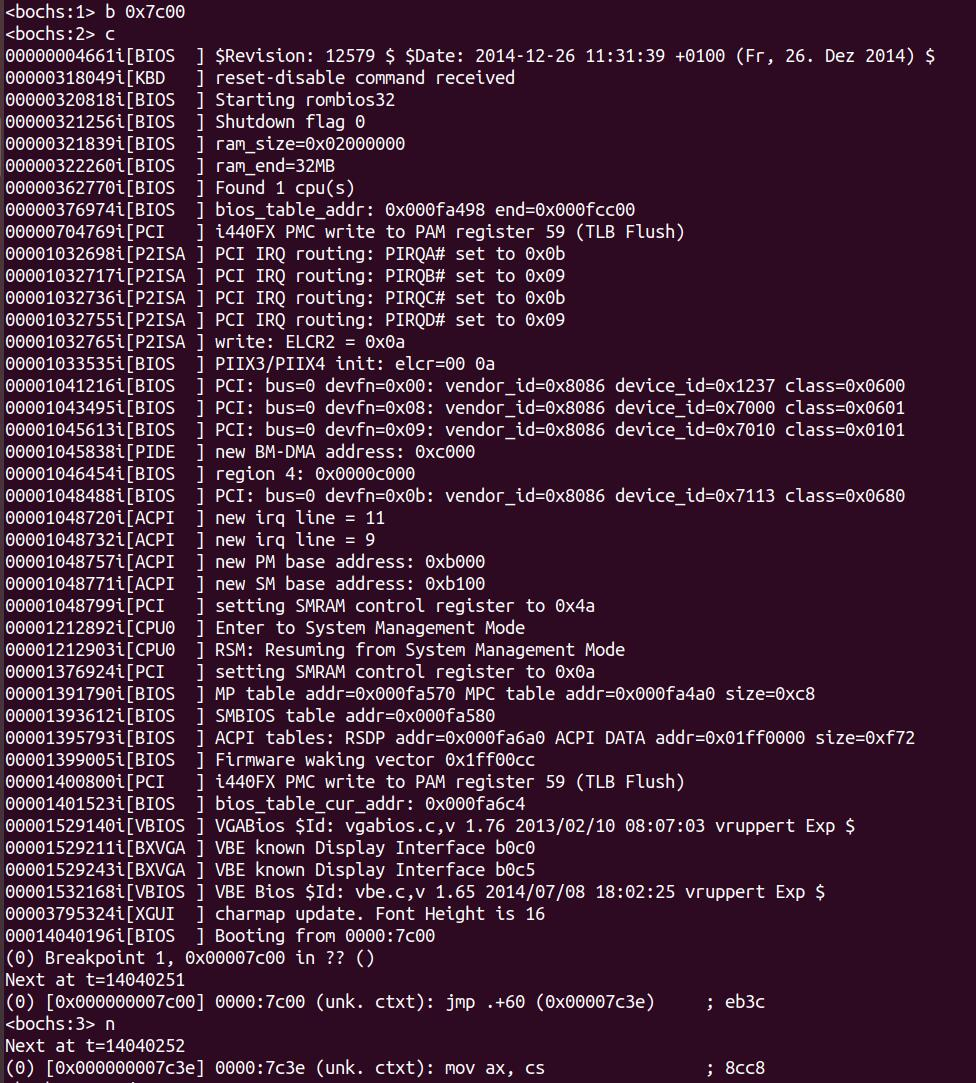
\includegraphics[width=0.8\textwidth]{figures/chapter5/5-2.jpg}
  \caption{调试过程 1}
  \label{fig:2}
\end{figure}

\begin{figure}[H]
  \centering
  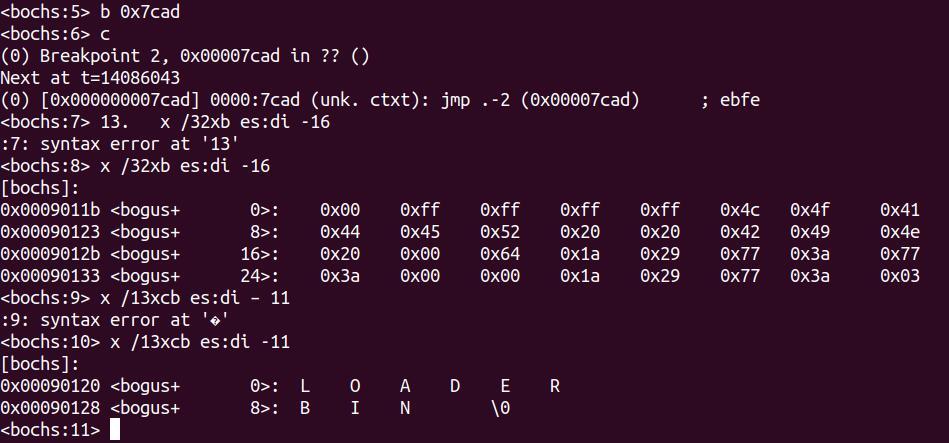
\includegraphics[width=0.8\textwidth]{figures/chapter5/5-3.jpg}
  \caption{调试过程 2}
  \label{fig:3}
\end{figure}

\begin{figure}[H]
  \centering
  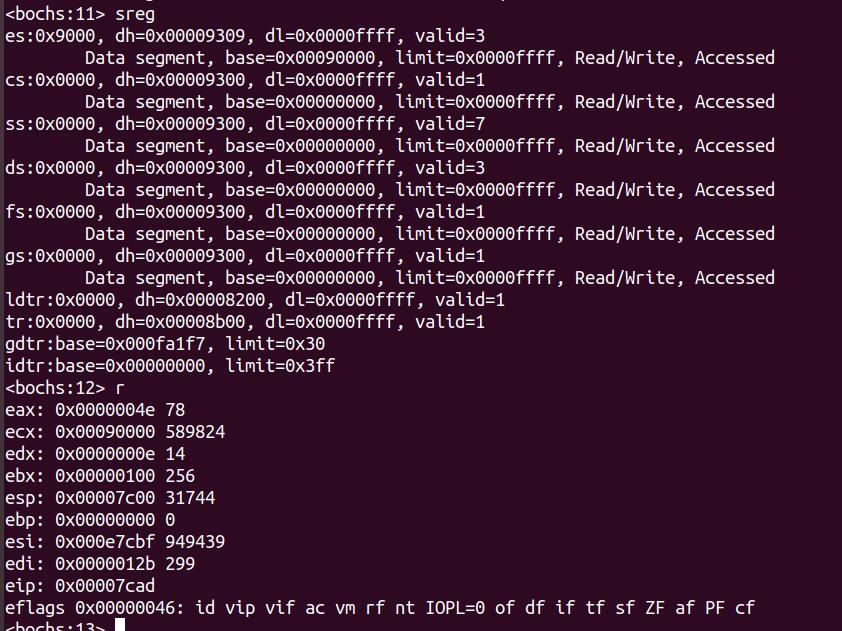
\includegraphics[width=0.8\textwidth]{figures/chapter5/5-4.jpg}
  \caption{调试过程 3}
  \label{fig:4}
\end{figure}

最后,再次修改boot.asm使其将控制权交给loader.bin。调试结果如下图5-5所示:
\begin{figure}[H]
  \centering
  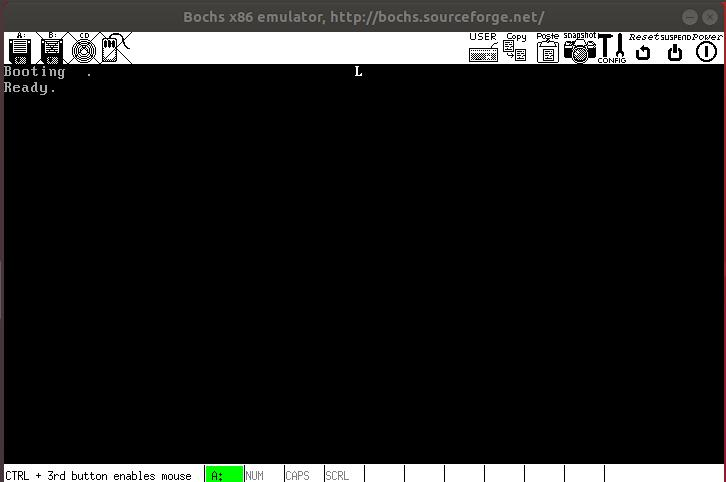
\includegraphics[width=0.8\textwidth]{figures/chapter5/5-5.jpg}
  \caption{控制权交给loader}
  \label{fig:5}
\end{figure}

\section{实验总结}
为突破 512 字节限制,我们进入保护模式的具体过程是:引导->加载内核入内存->跳入保护模式->开始执行内核,这样的工作如果全部交给引导扇区做,空间会不够,因此我们将其交给 Loader 模块完成,引导扇区负责把 Loader 载入内存并将控制权移交给它。我使用的软盘是FAT12 格式。FAT12 格式分为若干个扇区,引导扇区是整个磁盘的第 0 个扇区,在这个扇区中有一个重要数据结构 BPB,说明 FAT 的内容,之后则依次是 FAT1、FAT2、根目录区及数据区。而引导扇区需要有 BPB 等头信息才能被识别,故将其添加在boot.asm开头。\par
在本实验中,我们实现了 boot.asm ,使其可以从软盘中读出 Loader.bin文件,并且加载入内核,同时移交控制权。只要一个.COM 文件中不含有 DOS 系统调用,我们就可以将它当成 Loader 使用,现在的程序已经可以被看做是一个在保护模式下执行的“操作系统”了。但是,我们目前的 Loader 仅仅只是一个 Loader,它不是操作系统内核,也不能当做操作系统内核,操作系统内核应该至少可以在 Linux 下用 GCC 编译链接,摆脱汇编语言,而 Loader 至少要实现两个功能:将内核加载入内存和跳入保护模式。

\chapter{内核雏形}\label{cha:latex-brief-intro}

\section{实验内容}
进程切换;丰富中断处理程序,比如让时钟中断处理可以不停地发生而不是只发生一次,进程状态的保存与恢复,进程调度,解决中断重入问题。

\section{代码分析}

\subsection{核心数据结构}

\begin{table}[H]
\begin{center}
\caption{主要数据结构}
\begin{tabular}{|c|l|l|}
\hline
\multirow{2}{*}{结构体} & STACK\_FRAME       & 进程表结构体的定义 \\ \cline{2-3} 
                     & PROCESS            & 进程结构体的定义  \\ \hline
\multirow{2}{*}{宏}   & NR\_TASKS          & 最大允许进程:1  \\ \cline{2-3} 
                     & STACK\_SIZE\_TOTAL & 栈的大小      \\ \hline
\end{tabular}
\end{center}
\end{table}


\subsection{关键代码分析}
\begin{enumerate}
    \item \texttt{[section .text]}
    \texttt{global \_start}:让\texttt{\_start}符号成为可见的标识符,这样链接器就知道跳转到程序中的什么地方并开始执行程序。
    \texttt{\_start}:
    设置参数三:字符串长度
    设置参数二:要显示的字符串
    设置参数一:文件描述符(\texttt{stdout})

    \item 系统调用号(\texttt{sys\_write}):调用内核功能进行写操作
    系统调用号(\texttt{sys\_exit}):调用内核功能进行退出操作
    
    \item \texttt{[section .text]}
    外部函数\texttt{extern choose}
    \texttt{\_start}:
    将\texttt{num2nd}和\texttt{num1st}推入栈中
    调用外部函数\texttt{choose}
    增加栈指针8个字节
    系统调用号(\texttt{sys\_exit}):调用内核功能进行退出操作

    \item \texttt{myprint}函数:设置参数二:\texttt{len},设置参数一:\texttt{msg}
    设置参数:文件描述符(\texttt{stdout})
    
    \item 系统调用号(\texttt{sys\_write}):调用内核功能进行写操作

    \item 文件\texttt{bar.c}:
    声明外部函数\texttt{myprint()}
    定义\texttt{choose()}函数
    若\texttt{a >= b}:
    调用\texttt{myprint}输出"the 1st one"
    否则:
    调用\texttt{myprint}输出"the 2nd one"
    
    \item 文件\texttt{loader.asm}
    
    \item 使\texttt{ds}、\texttt{es}、\texttt{ss}三个段寄存器指向与\texttt{cs}相同的段,设置栈指针\texttt{sp}指向栈底

    \item 清屏并显示字符串"Booting"

    \item 软驱复位

    \item 在A盘的根目录中查找\texttt{LOADER.BIN}:遍历根目录,加载每个扇区到内存中,然后从中寻找文件名为\texttt{Loader.bin}的条目,直到找到为止。每读取一个扇区,在"Booting"后面打一个点。在成功加载和执行后显示字符串"Ready"。将控制权正式转移到已加载到内存中的\texttt{LOADER.BIN}的开头,开始执行其代码。

    \item \texttt{DispStr}函数:显示一个字符串

    \item \texttt{ReadSector}函数:从第\texttt{ax}个扇区开始,将\texttt{cl}个扇区读入\texttt{es:bx}中

    \item \texttt{GetFATEntry}函数:在FAT中找到序号为\texttt{ax}的扇区的条目,结果存储在\texttt{ax}中。需要注意的是,在过程中需要将FAT扇区读入\texttt{es:bx},因此函数开始时保存了\texttt{es}和\texttt{bx}。

    \item \texttt{KillMotor}函数:关闭软驱马达
    
    \item 文件\texttt{Kernel.asm}:
    \texttt{[section .text]}
    \texttt{global \_start};导出\texttt{\_start}
    跳转到\texttt{\_start},假设\texttt{gs}指向视频内存。设置黑底白字。设置\texttt{AL='K'}。在\texttt{gs}的偏移位置(屏幕第1行39列)写入字符'L'。
    无限循环。
    
    \item 文件\texttt{loader.asm}:
    重新整理和对齐\texttt{KERNEL.BIN}的内容,将其放置在一个新位置。迭代每个程序头,根据程序头中的信息确定将什么内容放入内存中,放在何处,以及放置多少。
\end{enumerate}


\section{调试过程及结果分析}
调试时主要出现以下问题,运行链接指令:ld -s hello.o -o hello报错,查阅资料后得知该指令只适用于 32 位操作系统的环境,而我们现在使用的操作系统为 64 位。因此修改为:ld -m elf$\_$i386 -o hello hello.o,修改后成功运行,结果如下图6-1所示:
\begin{figure}[H]
  \centering
  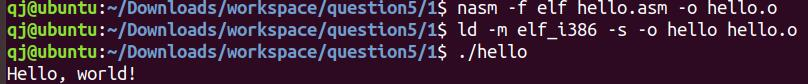
\includegraphics[width=0.8\textwidth]{figures/chapter6/6-1.jpg}
  \caption{汇编语言 Hello World 运行结果 }
  \label{fig:1}
\end{figure}

同样地,在编译时也需要指定32位的方式,使用以下指令:gcc -m32 -c -o bar.o bar.c。foobar运行结果如下图6-2所示:
\begin{figure}[H]
  \centering
  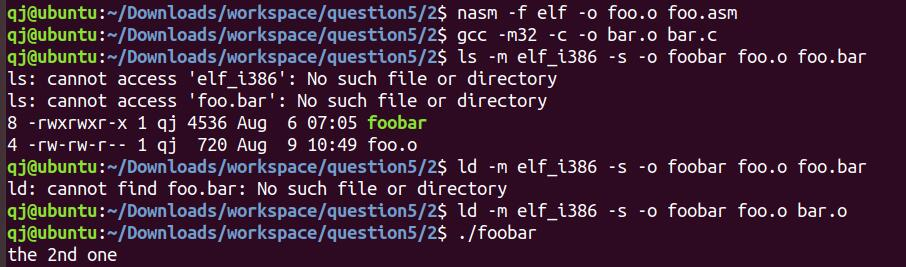
\includegraphics[width=0.8\textwidth]{figures/chapter6/6-2.jpg}
  \caption{foobar 执行结果}
  \label{fig:2}
\end{figure}

在此处,定义了 num1=3,num2=4,程序输出大的那个数的结果,可以看到,程序输出了“the 2nd one”的字样,成功完成了任务。接着,我们以同样方式编译boot,loader和kernel,调试运行结果如下图6-3所示:
\begin{figure}[H]
  \centering
  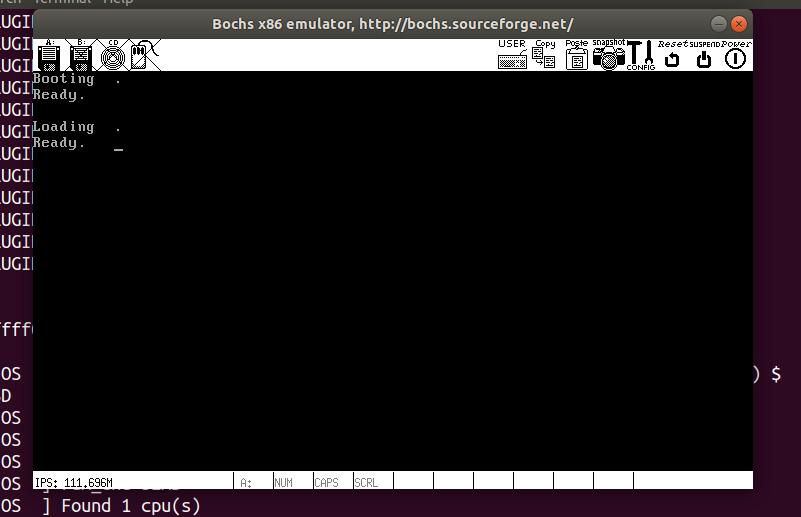
\includegraphics[width=0.8\textwidth]{figures/chapter6/6-3.jpg}
  \caption{载入内核}
  \label{fig:3}
\end{figure}

可以看到,在上一个实验的基础上,这次的实验结果多出了“Loading……”及“Ready.”这样的两行,说明我们已经载入了内核,并且由 Loader 读取了扇区。此外,还要将控制权交给内核,并重新进行调试,结果如下图6-4所示:
\begin{figure}[H]
  \centering
  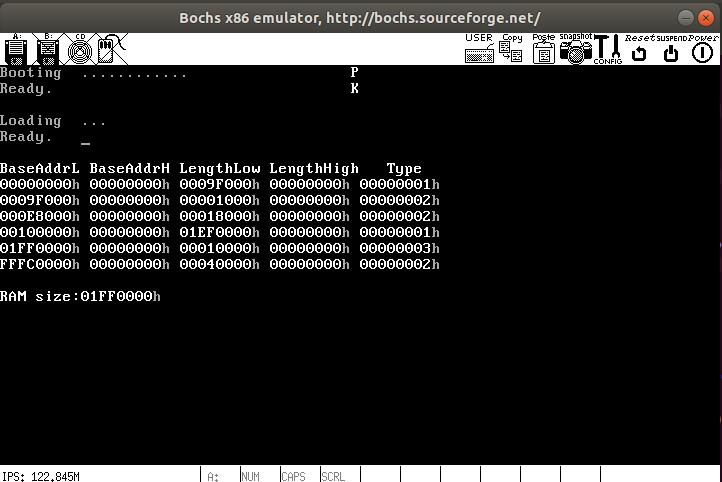
\includegraphics[width=0.8\textwidth]{figures/chapter6/6-4.jpg}
  \caption{控制权交给内核}
  \label{fig:4}
\end{figure}

\section{实验总结}
在本实验中,我们的程序定义了两个节(Section),一个放数据,一个放代码。在代码中值得注意的一点是,入口点默认的是“$\_$start”,在定义它之后还要通过 global 这个关键字让连接程序找到它。代码本身则利用了两个系统调用。\par
实验要结合本机的环境进行,书上使用的是 32 位虚拟机,而现在的Ubuntu更多地是 64 位环境,因此需要针对这一点进行更改。\par
另一方面 ,本章节所实现的操作系统内核已经达到可以使用高级语言程序的地步了,这使得我们后面增加新功能的时候更加方便,可以更多地使用我们更习惯的c语言而不需要再去写底层的汇编语言。除此之外我们也为后面使用 Makefile 文件做好了铺垫,以便我们可以免去那些繁杂重复的工作。这个章节操作和实现上均较简单,但是是意义重大的承上启下的一步——我们将进入保护模式的复杂操作交给了内核,以后这些重复性工作将由内核替我们完成。\par



\chapter{进程与进程调度}\label{cha:latex-brief-intro}

\section{实验内容}
进程切换;丰富中断处理程序,比如让时钟中断处理可以不停地发生而不是只发生一次,进程状态的保存与恢复,进程调度,解决中断重入问题。

\section{代码分析}

\subsection{核心数据结构}

\begin{table}[H]
\begin{center}
\caption{主要数据结构}
\begin{tabular}{|c|l|l|}
\hline
\multirow{2}{*}{结构体} & STACK\_FRAME       & 进程表结构体的定义 \\ \cline{2-3} 
                     & PROCESS            & 进程结构体的定义  \\ \hline
\multirow{2}{*}{宏}   & NR\_TASKS          & 最大允许进程  \\ \cline{2-3} 
                     & STACK\_SIZE\_TOTAL & 栈的大小      \\ \hline
\end{tabular}
\end{center}
\end{table}


\subsection{关键代码分析}

\begin{enumerate}
    \item 进程切换,实现从 Ring 0 到 Ring 1 的切换:\par
        当发生中断时,从内核栈切换到进程栈,指向就绪队列中下一个应该被执行的进程,同时用 TSS 保存 Ring 0 的信息,如图 7-1 所示:
        \begin{lstlisting}[language = C]
          mov  esp, [p_proc_ready]    
          lldt [esp + P_LDT_SEL]
          lea  eax, [esp + P_STACKTOP]
          mov  dword [tss + TSS3_S_SP0], eax
        \end{lstlisting}
        
        取出下一个进程所需的寄存器值,利用 \texttt{iretd} 转到 Ring 1 特权级,执行该进程,如下所示:
        \begin{lstlisting}[language = C]
          pop  gs
          pop  fs
          pop  es
          pop  ds
          popad
          add  esp, 4
          iretd
        \end{lstlisting}
    
    \item 丰富中断处理程序,让时钟中断处理可以不停发生,并在进行进程调度的时候做到进程的保存与恢复。让中断可以不停发生,设置 EOI,如下所示:
    \begin{lstlisting}[language = C]
    hwint00:
      mov  al, EOI
      out  INT_M_CTL, al
      iretd
    \end{lstlisting}
    
    为了让被中断的进程能够顺利恢复,在进程表中,我们给每一个寄存器预留了位置,以便让他们把所有的值都保存下来,这样在进程切换的时候就不会对进程产生不良影响。使用 \texttt{push} 保存原寄存器值,如下所示:
    \begin{lstlisting}[language = C]
      pushad
      push  ds
      push  es
      push  fs
      push  gs
    \end{lstlisting}
    
    使用 \texttt{pop} 恢复原寄存器值,如下所示:
    \begin{lstlisting}[language = C]
      pop  gs
      pop  fs
      pop  es
      pop  ds
      popad
    \end{lstlisting}

    
    为了保存内核栈信息,在从 Ring 0 到 Ring 1 的时候,我们使用 TSS 保存 Ring 0 的信息。在每一次重新开始前,使用 \texttt{iretd} 返回 Ring 1 之前,我们都要进行检查,以确保 \texttt{tss.esp0} 是正确的,如下所示:
    \begin{lstlisting}[language = C]
      lea  eax, [esp + P_STACKTOP]
      mov  dword [tss + TSS3_S_SP0], eax
    \end{lstlisting}
    
    \item 解决中断重入问题:
    如果中断处理完成之前就会有下一个中断产生,我们会发现中断一直在进行,不会回到我们的程序。为解决中断重入问题,我们在 \texttt{main.c} 中设置全局变量 \texttt{k\_reenter}。该全局变量初值为 -1,中断处理程序开始执行时它自加,结束时自减。在处理程序开头处,这个变量需要被检查一下,如果值不是 0,则说明在一次中断未处理完之前就又发生了一次中断,这时直接跳到最后,结束中断处理程序的执行。然后判断是否需要跳转,如果 \texttt{k\_reenter} 不为 0,则直接结束当前中断,恢复上一个进程的执行,如下所示:
    \begin{lstlisting}[language = C]
      k_reenter = -1;
    \end{lstlisting}
    
    \begin{lstlisting}[language = C]
      inc  dword [k_reenter]
      cmp  dword [k_reenter], 0
      jne  .re_enter
    \end{lstlisting}
    
    \begin{lstlisting}[language = C]
    .re_enter:
      dec  dword [k_reenter]
      pop  gs
      pop  fs
      pop  ds
      popad
      add  esp, 4
      iretd
    \end{lstlisting}
    
    \item 进程调度:
    发生时钟中断时选择进程表中的下一个进程来执行,现在我们希望设定进程的优先级。为每个进程添加一个变量 \texttt{ticks},初始值为进程的优先级。每次进程获得一个运行周期,\texttt{ticks} 减 1,减到 0 时,此进程不再获得执行机会,直到所有进程的 \texttt{ticks} 都减为 0。首先定义变量,如下所示:
    \begin{lstlisting}[language = C]
      proc_table[0].ticks = proc_table[0].priority = 150;
      proc_table[1].ticks = proc_table[1].priority = 50;
      proc_table[2].ticks = proc_table[2].priority = 30;
    \end{lstlisting}
    
    然后编写进程调度函数
    \texttt{schedule()},放在 \texttt{proc.c} 中,如下所示:
    \begin{lstlisting}[language = C]
    PUBLIC  void  schedule(){
      PROCESS* p;
      int  greatest_ticks = 0;
      while (!greatest_ticks){
        for (p = proc_table; p < proc_table + NR_TASKS; p++){
          if (p -> ticks > greatest_ticks){
            greatest_ticks = p -> ticks;
            p_proc_ready = p;
          }
          if (!greatest_ticks){
            for (p = proc_table; p < proc_table + NR_TASKS; p++){
              p ->ticks = p-> priority;
            }
          }
        }
      }
    }
    \end{lstlisting}
    
    同时修改时钟中断处理,如下所示:
    \begin{lstlisting}[language = C]
    PUBLIC  void  clock_handler(int irq){
      ticks++;
      p_proc_ready -> ticks++;
      if (k_reenter != 0){
        return;
      }
      schedule();
    }
    \end{lstlisting}
\end{enumerate}


\section{调试过程及结果分析}
由于使用的是64位系统,与参考书版本不一致,需对Makefile作一定修改:\par
CFLAGS	= -I include/ -c -fno-builtin LDFLAGS	= -s -Ttext \$(ENTRYPOINT)\par
DASMFLAGS	= -u -o \$(ENTRYPOINT) -e \$(ENTRYOFFSET)\par
改为:\par
CFLAGS	= -m32 -I include/ -c -fno-builtin -fno-stack-protector LDFLAGS	= -m elf$\_$i386 -s -Ttext \$(ENTRYPOINT)\par
DASMFLAGS	= -u -o \$(ENTRYPOINT) -e \$(ENTRYOFFSET) -m32\par
即可使用make指令直接完成编译等工作,后续调试方法与之前实验一致,进程切换实验结果如下图7-1所示:
\begin{figure}[H]
  \centering
  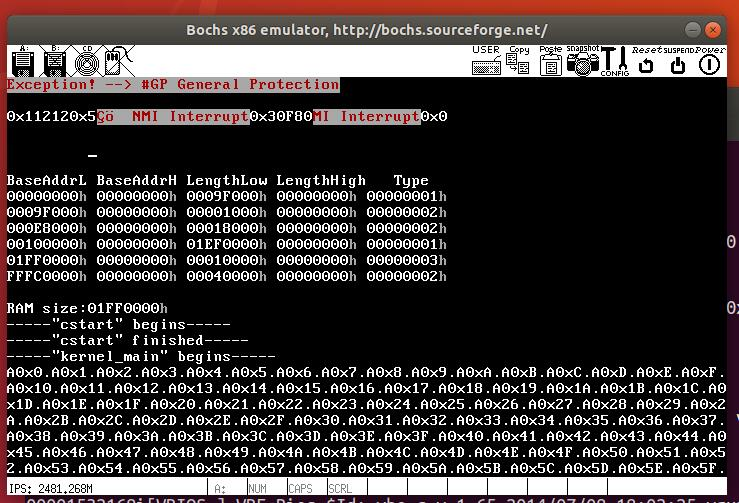
\includegraphics[width=0.8\textwidth]{figures/chapter7/7-1.jpg}
  \caption{进程切换实验结果}
  \label{fig:1}
\end{figure}

接着丰富中断处理程序,让时钟中断处理可以不停地发生而不是只发生一次,如下图7-2所示:
\begin{figure}[H]
  \centering
  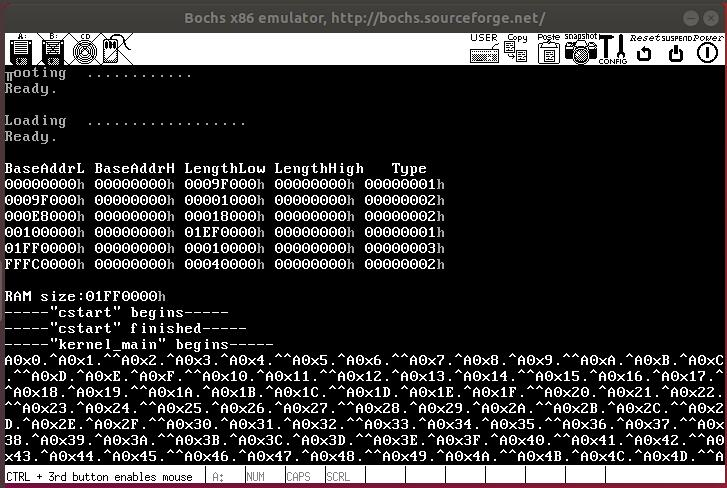
\includegraphics[width=0.8\textwidth]{figures/chapter7/7-2.jpg}
  \caption{中断不停发生实验结果}
  \label{fig:2}
\end{figure}

再实现进程状态的保存与恢复,如下图7-3所示:
\begin{figure}[H]
  \centering
  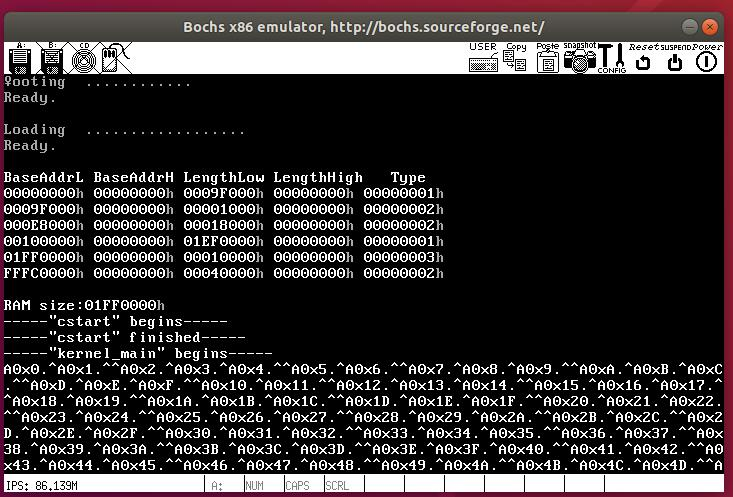
\includegraphics[width=0.8\textwidth]{figures/chapter7/7-3.jpg}
  \caption{中断不停发生实验结果}
  \label{fig:3}
\end{figure}

然后支持中断重入,如下图7-4所示:
\begin{figure}[H]
  \centering
  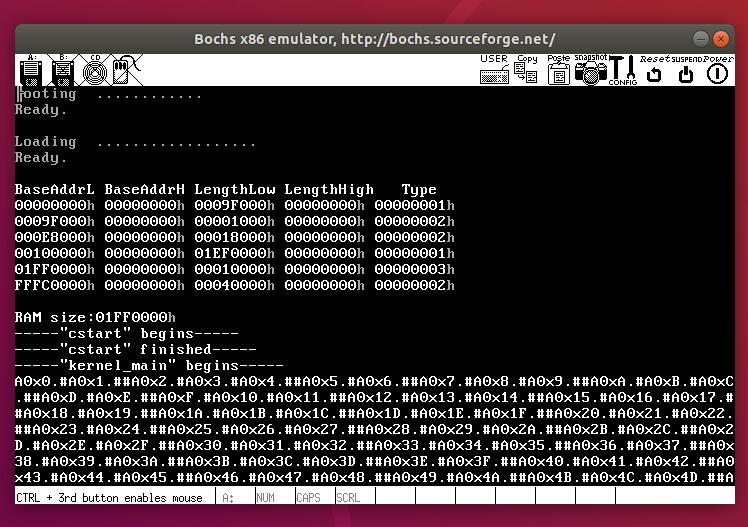
\includegraphics[width=0.8\textwidth]{figures/chapter7/7-4.jpg}
  \caption{中断重入实验结果}
  \label{fig:4}
\end{figure}

最后执行进程调度,如下图7-5所示:
\begin{figure}[H]
  \centering
  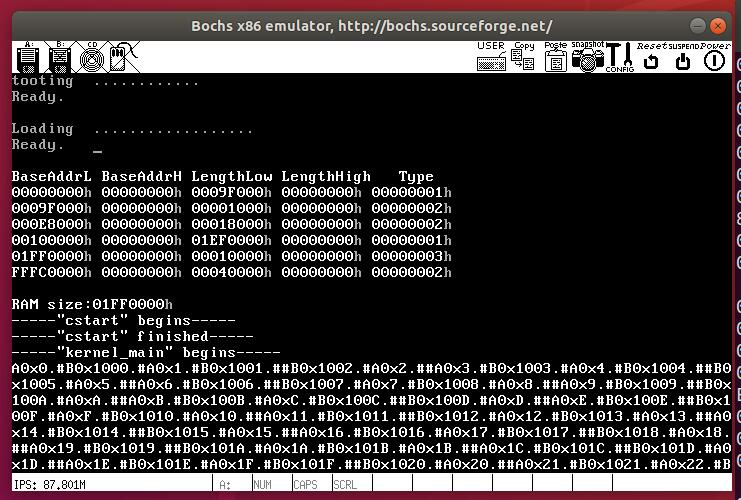
\includegraphics[width=0.8\textwidth]{figures/chapter7/7-5.jpg}
  \caption{进程调度实验结果}
  \label{fig:5}
\end{figure}

\section{实验总结}
本实验将重点放到了进程上。从进程切换,中断处理程序的丰富,再到进程切换时进程状态的保存与恢复,最后到进程调度,同时考虑并解决了中断重入问题。虽然还没办法进行输入输出,但已经可以说这个操作系统已经是一个基本完善的操作系统了。\par
本次实验使用了 Makefile 来化简我们的操作步骤以及展现不一样的内核效果。操作途中遇到了 Makefile 需要更改的问题,因为里面的内容是以 32 位虚拟机为对象来做的,而我们使用的是 64位虚拟机,将对应代码更改完后直接运行make指令,后续实验步骤和之前相同。\par
总而言之,第六个实验的任务是实现进程和进程调度。首先准备好进程体,初始化相应的描述符,准备进程表,完成特权级别的跳转,从 ring0 到 ring1。接下来要完善时钟中断处理程序,为此我们需要设置 EOI,运行可以看到 0行 0 列的字符不断变化,说明中断处理程序正在运行。然后是现场的保护和恢复,我们需要用进程表保存进程的状态,具体需要保存各寄存器的值,切内核栈和重新将 esp 切到进程表。然后是中断重入,如果中断未处理完之前又发生中断,直接结束中断处理程序的运行。实现多进程时,我们读取不同的任务地址入口、堆栈栈顶和进程名,在进程切换时重新加载 ldtr。进程切换时,为 esp 赋不同的值。我们只打开时钟中断的时候,屏蔽掉时间中断,并进行相关系统调用。在进程调度中,我们设置不同的延迟,进行了简单的优先级设置。整理的实验六的思维导图如下:
\begin{figure}[H]
  \centering
  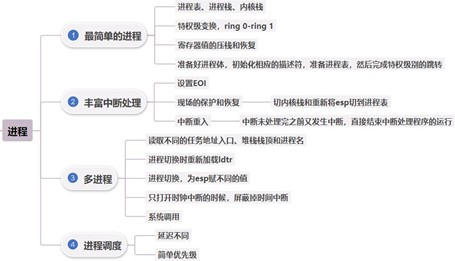
\includegraphics[width=0.8\textwidth]{figures/chapter7/7-6.jpg}
  \caption{实验六思维导图}
  \label{fig:6}
\end{figure}



\chapter{操作系统的输入/输入系统}\label{cha:latex-brief-intro}

\section{实验内容}
实现简单的 I/O,从键盘输入字符的中断开始;获取并打印扫描码;创建对应打印扫描码解析数组,打印对应字符。
\section{代码分析}

\subsection{核心数据结构}

\begin{table}[H]
\begin{center}
\caption{keyboard.h缓冲区KB$\_$INPUT}
\begin{tabular}{|c|l|l|}
\hline
\multirow{4}{*}{缓冲区 KB\_INPUT} & p\_head                & 指向缓冲区中下一个空闲位置 \\ \cline{2-3} 
                               & p\_tail                & 指向键盘任务应处理的字节  \\ \cline{2-3} 
                               & Count                  & 缓冲区中字节数       \\ \cline{2-3} 
                               & buf{[}KB\_IN\_BYTES{]} & 缓冲区           \\ \hline
\end{tabular}
\end{center}
\end{table}


\subsection{关键代码分析}
\begin{enumerate}

    \item 键盘中断处理程序:
    \begin{lstlisting}[language=C]
    PUBLIC void keyboard_handler(int irq)
    {
        disp_str("str");
    }
    \end{lstlisting}
    
    \item 打开键盘中断:
    \begin{lstlisting}[language=C]
    PUBLIC void init_keyboard()
    {
        put_irq_handler(KEYBOARD_IRQ, keyboard_handler); /* 设定键盘中断处理程序 */
        enable_irq(KEYBOARD_IRQ); /* 开启键盘中断 */
    }
    \end{lstlisting}
    
    \item 调用 \texttt{init\_keyboard}:
    \begin{lstlisting}[language=C]
    PUBLIC int kernel_main()
    {
        // ...
        init_keyboard();
        // ...
    }
    \end{lstlisting}
    
    \item 修改后的键盘中断:
    \begin{lstlisting}[language=C]
    PUBLIC void keyboard_handler(int irq)
    {
        /* disp_str("*"); */
        u8 scan_code = in_byte(0x60);
        disp_int(scan_code);
    }
    \end{lstlisting}
    
    \item 扫描码解析数组:
    \begin{lstlisting}[language=C]
    u32 keymap[NR_SCAN_CODES * MAP_COLS] = {
        /* 0x00 - none */ 0, 0, 0,
        /* 0x01 - ESC */ ESC, ESC, 0,
        /* 0x02 - '1' */ '1', '!', 0,
        // ...
    };
    \end{lstlisting}
    
    \item 键盘缓冲区:
    \begin{lstlisting}[language=C]
    typedef struct s_kb {
        char* p_head;   /* 指向缓冲区中下一个空闲位置 */
        char* p_tail;   /* 指向键盘任务应处理的字节 */
        int count;      /* 缓冲区中共有多少字节 */
        char buf[KB_IN_BYTES]; /* 缓冲区 */
    } KB_INPUT;
    \end{lstlisting}
    
    \item 修改后的 \texttt{keyboard\_handler}:
    \begin{lstlisting}[language=C]
    PRIVATE KB_INPUT kb_in;
    
    /* keyboard_handler */
    PUBLIC void keyboard_handler(int irq)
    {
        u8 scan_code = in_byte(KB_DATA);
        if (kb_in.count < KB_IN_BYTES) {
            *(kb_in.p_head) = scan_code;
            kb_in.p_head++;
            if (kb_in.p_head == kb_in.buf + KB_IN_BYTES) {
                kb_in.p_head = kb_in.buf;
            }
            kb_in.count++;
        }
    }
    \end{lstlisting}
    
    \item 修改后的 \texttt{init\_keyboard}:
    \begin{lstlisting}[language=C]
    PUBLIC void init_keyboard()
    {
        kb_in.count = 0;
        kb_in.p_head = kb_in.p_tail = kb_in.buf;
        put_irq_handler(KEYBOARD_IRQ, keyboard_handler); /* 设定键盘中断处理程序 */
        enable_irq(KEYBOARD_IRQ); /* 开键盘中断 */
    }
    \end{lstlisting}
    
    \item 时钟中断处理函数 \texttt{init\_clock}:
    \begin{lstlisting}[language=C]
    PUBLIC void init_clock()
    {
        /* 初始化 8253 PIT */
        out_byte(TIMER_MODE, RATE_GENERATOR);
        out_byte(TIMER0, (u8) (TIMER_FREQ/HZ));
        out_byte(TIMER0, (u8) ((TIMER_FREQ/HZ) >> 8));
        put_irq_handler(CLOCK_IRQ, clock_handler); /* 设定时钟中断处理程序 */
        enable_irq(CLOCK_IRQ); /* 让 8259A 可以接收时钟中断 */
    }
    \end{lstlisting}
    
    \item 键盘读取的 \texttt{tty} 任务:
    \begin{lstlisting}[language=C]
    PUBLIC void task_tty()
    {
        while (1) {
            keyboard_read();
        }
    }
    \end{lstlisting}
    
    \item 键盘读取函数 \texttt{keyboard\_read()}:
    \begin{lstlisting}[language=C]
    PUBLIC void keyboard_read()
    {
        u8 scan_code;
        if (kb_in.count > 0) {
            disable_int();
            scan_code = *(kb_in.p_tail);
            kb_in.p_tail++;
            if (kb_in.p_tail == kb_in.buf + KB_IN_BYTES) {
                kb_in.p_tail = kb_in.buf;
            }
            kb_in.count--;
            enable_int();
            disp_int(scan_code);
        }
    }
    \end{lstlisting}
    
    \item \texttt{disable\_int} 与 \texttt{enable\_int}:
    \begin{lstlisting}[language=C]
    /* void disable_int(); */
    /* disable_int: */
    /* cli */
    /* ret */
    
    /* void enable_int(); */
    /* enable_int: */
    /* sti */
    /* ret */
    \end{lstlisting}
    
    \item 解析扫描码:
    \begin{lstlisting}[language=C]
    PUBLIC void keyboard_read()
    {
        u8 scan_code;
        char output[2];
        int make; /* TRUE: make; FALSE: break. */
    
        memset(output, 0, 2);
        if (kb_in.count > 0) {
            disable_int();
            scan_code = *(kb_in.p_tail);
            kb_in.p_tail++;
            if (kb_in.p_tail == kb_in.buf + KB_IN_BYTES) {
                kb_in.p_tail = kb_in.buf;
            }
            kb_in.count--;
            enable_int();
            /* 下面开始解析扫描码 */
            if (scan_code == 0xE1) {
                /* 暂时不做任何操作 */
            }
            else if (scan_code == 0xE0) {
                /* 暂时不做任何操作 */
            }
            else {
                /* 下面处理可打印字符 */
                /* 首先判断 Make Code 还是 Break Code */
                make = (scan_code & FLAG_BREAK ? FALSE : TRUE);
                /* 如果是 Make Code 就打印,是 Break Code 则不做处理 */
                if (make) {
                    output[0] = keymap[(scan_code & 0x7F) * MAP_COLS];
                    disp_str(output);
                }
            }
        }
    }
    \end{lstlisting}
\end{enumerate}


\section{调试过程及结果分析}
使用make指令编译,bochs指令运行,可以看到,当我们敲击键盘之后,程序中出现了一个“*”的字符,但当我们再次敲击键盘后,键盘却不会再次相应,即屏幕上不会出现第二个“*”字符,而且在terminal中可以看到栈溢出的报错信息。结果如下图8-1所示:
\begin{figure}[H]
  \centering
  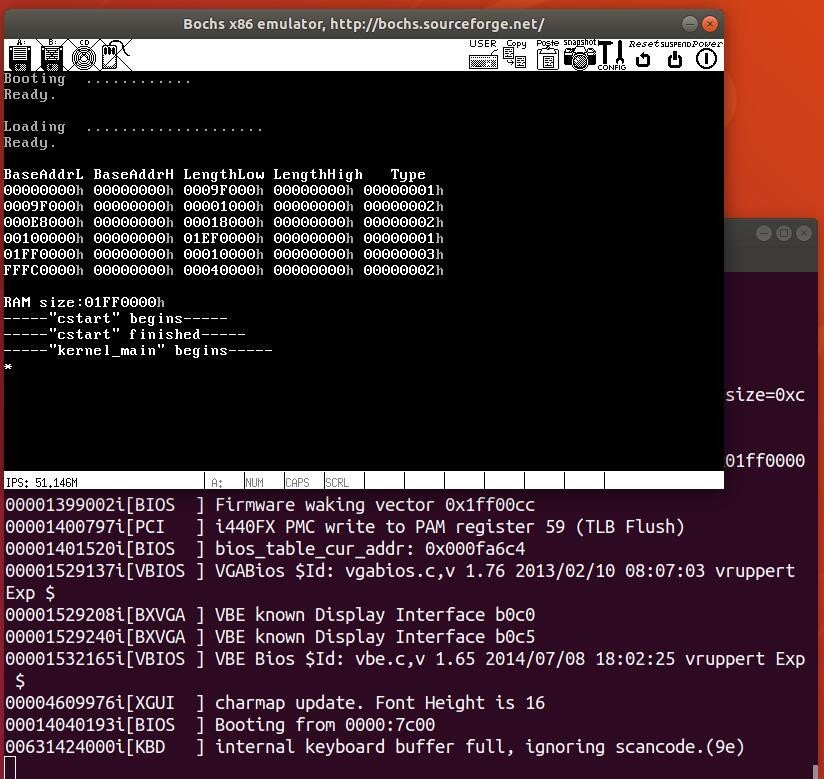
\includegraphics[width=0.8\textwidth]{figures/chapter8/8-1.jpg}
  \caption{键盘中断处理程序打印星号}
  \label{fig:1}
\end{figure}

在此处,我们调用键盘中断,在敲击键盘后出现了一个“*”字符,代表我们的键盘中断是准确无误的,但它目前只能相应一次键盘敲击。结合栈溢出的报错信息,我们可以每次输出缓冲区中字符对应的解析码。运行结果如下图8-2所示:
\begin{figure}[H]
  \centering
  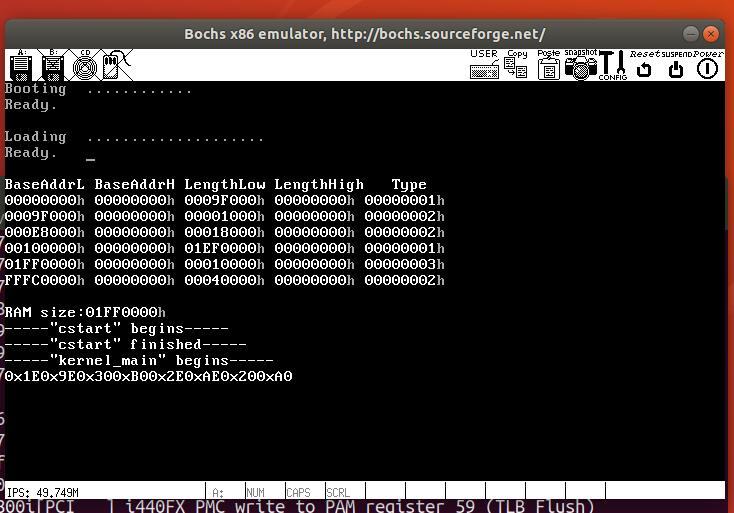
\includegraphics[width=0.8\textwidth]{figures/chapter8/8-2.jpg}
  \caption{读取缓冲区并打印解析码}
  \label{fig:2}
\end{figure}

在上图所示调试过程中,我们连续连续敲击了四个键:字符“a”、字符“b”、字符“c”和字符“d”,而实验结果则一共出现了 8 组数字,分别对应于字符“a”、“b”、“c”和“d”的 Make Code 和 Break Code。可以看到,我们目前的程序已经不会再卡死,而是可以相应多次键盘敲击过程,并且打印出扫描码。对于这一点,则涉及到键盘控制器 8042 芯片和键盘编码器 8048 芯片,它们会监视键盘的输入,并把适当的数据传给计算机。而对于敲击键盘的动作,则会产生扫描码,分别为按下一个按键或保持一个按键的 Make Code 和键盘弹起时的 Break Code,这些扫描码可以通过 in al,60h 读取,并且只有我们将扫描码从缓冲区中读出来后,8042 才能继续响应新的按键,这也解释了我们在之前的实验中只打印一个“*”的原因。接下来我们通过扫描码解析数组 keymap[ ],建立字符与解析码之间的映射关系,再次调试结果如下图8-3所示:
\begin{figure}[H]
  \centering
  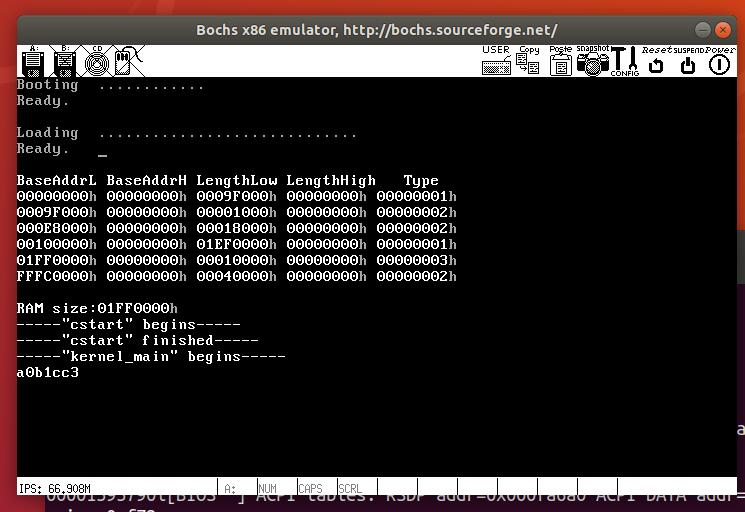
\includegraphics[width=0.8\textwidth]{figures/chapter8/8-3.jpg}
  \caption{输出正确的小写字符和数字}
  \label{fig:3}
\end{figure}

可以看到,目前我们的程序已经可以对小写 a-z 以及 0-9 产生正常响应,但仍然无法打印出大写字母,对 shift、alt、ctrl等按键则会输出意义不明的字符。由于我们已经知晓键盘敲击产生字符的原理,根据组合键的Make Code和Break Code专门处理,这一点不难实现。实现后运行结果如下图8-4所示:
\begin{figure}[H]
  \centering
  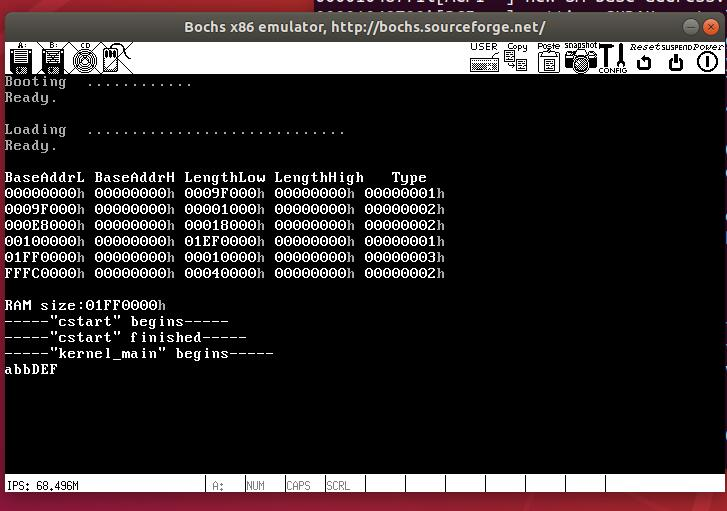
\includegraphics[width=0.8\textwidth]{figures/chapter8/8-4.jpg}
  \caption{输出组合键}
  \label{fig:4}
\end{figure}

\section{实验总结}

本次实验研究的是输入与输出。经过这次实验,我对电脑如何将外界输入处理成对应显示有了更深的了解。一次按键对应一个输出字符很好理解,但对于各种复杂组合键的实现方法,了解到敲击键盘按下和松开分别会有两个扫描码后,这才从原理上完全理解。\par
总而言之,第七个实验的任务是实现操作系统的输入输出系统。最初的时候,我们的键盘只能输入一个星号,因为这个程序并没有从缓冲区读取扫描码,相应的芯片不能及时响应按键。然后我们添加 in$\_$byte(0x60)指令,这样就可以多次输入了。接着,我们再次修改代码,使得屏幕能够显示按键的扫描码 MakeCode 和 BreakCode。接下来,我们引入扫描码解析数组,再使用键盘缓冲区存放暂未处理的输入。我们首先忽略 0xE0 和 0xE1。这样所有的小写字母就可以正常输出了。然后增加处理 Shift 的代码,这样就能够识别大写字母和特殊字符了。整理的实验七实验思维导图如下图 8-5 所示:
\begin{figure}[H]
  \centering
  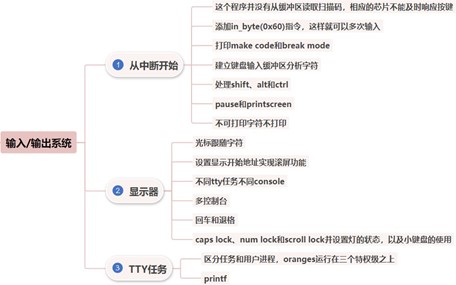
\includegraphics[width=0.8\textwidth]{figures/chapter8/8-5.jpg}
  \caption{实验七思维导图}
  \label{fig:5}
\end{figure}

\chapter{操作系统进阶}\label{cha:latex-brief-intro}

\section{实验内容}
\begin{enumerate}
    \item 自定义一个系统调用,能够统计一个进程在执行的过程中被调度的次数。编写一个简单的用户程序,调用该自定义的系统调用,从而将进程及其调度的次数输出在屏幕上。
    \item 在实现了三个进程的优先级调度的基础上,将三个进程的循环次数从无限循环修改为有限次数,当三个进程执行完成时,计算三个进程在优先级调度算法下的周转时间、等待时间以及该系统的平均周转时间、平均等待时间和吞吐量。也可以添加新的进程,然后计算该系统的平均周转时间、平均等待时间和吞吐量。
\end{enumerate}

\section{代码分析}

\subsection{系统调用部分}
    \begin{enumerate}
        \item 系统调用过程:(以书中 write 系统调用为例),如下图 9-1 所示:
        \begin{figure}[H]
            \centering
            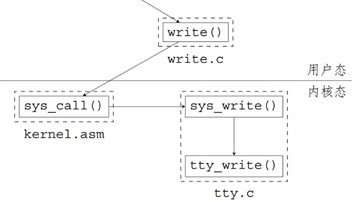
\includegraphics[width=0.8\textwidth]{figures/chapter9/9-1.jpg}
            \caption{系统调用流程图}
        \end{figure}
        
        \item 实现一个新的系统调用(这里为 get$\_$foo)主要需要完成两部分:get$\_$foo函数本身 及其内核部分 sys$\_$get$\_$foo,如图 9-2 所示:
        \begin{figure}[H]
            \centering
            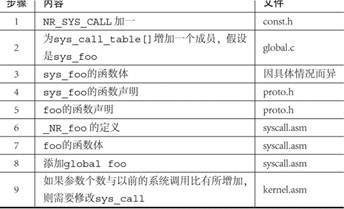
\includegraphics[width=0.8\textwidth]{figures/chapter9/9-2.jpg}
            \caption{系统调用函数}
        \end{figure}
        
        \item 添加系统调用的步骤:
        \begin{enumerate}
            \item 将 \texttt{const.h} 文件中的宏 \texttt{NR\_SYS\_CALL} 加 1。\\
            \texttt{NR\_SYS\_CALL} 表示的是操作系统中定义的系统调用的个数,会用到其值来定义系统调用数组。
            
            \item 在 \texttt{global.c} 文件为 \texttt{sys\_call\_table[]} 增加一个成员,命名为sys$\_$get$\_$foo,此处模仿前两个系统调用名并结合功能设为 \texttt{sys\_get\_num}。此处用到了步骤一中设置的 \texttt{NR\_SYS\_CALL} 来定义数组。
            
            \item 完成 \texttt{get\_foo} 的声明及 \texttt{sys\_get\_foo} 的声明和函数体。声明位于头文件 \texttt{proto.h} 中,函数体的位置较灵活,此处选择将新增的系统调用放在第一个系统调用 \texttt{sys\_get\_ticks} 后面,即 \texttt{proc.c} 文件最下方。
            
            \item 定义 \texttt{\_NR\_get\_foo} 及添加 \texttt{global get\_foo}。\\\texttt{\_NR\_get\_time equ} 后的值设为1,和已有系统调用的调用号不一致即可。
            
            \item 设计用户程序:在 \texttt{main.c} 文件中编写了测试进程:\texttt{TestA}、\texttt{TestB} 与 \texttt{TestC},如图所示。其中,\texttt{TestA} 调用了 \texttt{get\_foo} 与 \texttt{get\_ticks} 系统调用函数,进程 \texttt{B} 与进程 \texttt{C} 没有调用系统函数,目的为与 \texttt{TestA} 形成对照,使实验结果清晰,如下所示:
            \begin{lstlisting}[language = C]
    void TestA(){
        for(int k = 0;k < 10;k++){
        disp_str("A");
        disp_int(get_foo() + 1);
        disp_int(get_ticks());
        milli_delay(100);
        }
    }
            \end{lstlisting}
            \begin{lstlisting}[language = C]
    void TestB(){
        for(int i = 0;i < 10;i++){
        disp_str("B");
        milli_delay(100);
        }
    }
            \end{lstlisting}
            \begin{lstlisting}[language = C]
    void TestC(){
        for(int i = 0;i < 10;i++){
        disp_str("C");
        milli_delay(100);
        }
    }
            \end{lstlisting}
        \end{enumerate}
    \end{enumerate}


\subsection{优先级调度部分}
\begin{enumerate}
        \item 此处添加用户进程的主要步骤与系统调用部分完全一致,不重复阐述。
        
        \item 在 \texttt{main.c} 文件中给三个进程添加ticks属性,定义为有限值,每次调用ticks值减一,为0后则不再调用。并对proc.c文件中的schedule函数进行修改,删掉ticks归零后重新赋值的部分,从而将三个进程的循环次数从无限循环修改为有限次数。如下所示:
\begin{lstlisting}[language = C]
    proc_table[0].ticks = 100;
    proc_table[1].ticks = 40;
    proc_table[2].ticks = 30;
\end{lstlisting}

\begin{lstlisting}[language = C]
    /*if (!greatest_ticks){
        for (p = proc_table; p < proc_table + NR_TASKS; p++){
        p ->ticks = p-> priority;
        }
    }*/
\end{lstlisting}
        
        \item 在进程结构体中添加相应成员。周转时间命名为 \texttt{TurnaroundTick},等待时间命名为\texttt{WaitingTick}。
        此处,我对优先级调度算法进行了修改,使进程调度完全按照自行设定的优先级顺序(priority值的大小)来执行,保证高优先级进程一定在低优先级进程之前执行完毕。因此,周转时间直接读取进程结束时的ticks中,而等待时间可直接读取进程开始时的ticks。调度算法如下:
\begin{lstlisting}[language = C]
    PROCESS*	p;
    int		greatest_priority = 0;
    for (p=proc_table; p<proc_table+NR_TASKS; p++) {
		if (p->priority > greatest_priority && p->ticks > 0) {
			greatest_priority = p->priority;
			p_proc_ready = p;
		}
    }
\end{lstlisting}
        
        \item 三个进程结束后计算并打印出相应的数据,需要注意的是单位为ms,要进行转换。如下所示:
\begin{lstlisting}[language = C]
if (greatest_priority == 0) {
    // turnaround time
    disp_str("\n");
    disp_str("turnaround time of a:");
    disp_int(proc_table[0].TurnaroundTick /  10);
    disp_str("ms\n");

    disp_str("turnaround time of b:");
    disp_int(proc_table[1].TurnaroundTick /  10);
    disp_str("ms\n");

    disp_str("turnaround time of c:");
    disp_int(proc_table[2].TurnaroundTick /  10);
    disp_str("ms\n");

    // waiting time
    disp_str("waiting time of a:");
    disp_int(proc_table[0].WaitingTick /  10);
    disp_str("ms\n");

    disp_str("waiting time of b:");
    disp_int(proc_table[1].WaitingTick /  10);
    disp_str("ms\n");

    disp_str("waiting time of c:");
    disp_int(proc_table[2].WaitingTick /  10);
    disp_str("ms\n");

    // average turnaround time
    disp_str("average turnaround time:");
    disp_int((proc_table[0].TurnaroundTick + proc_table[1].TurnaroundTick + proc_table[2].TurnaroundTick / 30) / 30);
    disp_str("ms\n");
    disp_str("average waiting time:");
    disp_int((proc_table[0].WaitingTick + proc_table[1].WaitingTick + proc_table[2].WaitingTick) / 30);
    disp_str("ms\n");

    // throughput
    disp_str("throughput:");
    int timeOfThree = proc_table[0].TurnaroundTick > proc_table[1].TurnaroundTick ? proc_table[0].TurnaroundTick : proc_table[1].TurnaroundTick;
    timeOfThree = timeOfThree > proc_table[2].TurnaroundTick ? timeOfThree : proc_table[2].TurnaroundTick;
    disp_int((proc_table[0].ticks + proc_table[1].ticks + proc_table[2].ticks)/ timeOfThree);
    disp_str("/s\n");
}
\end{lstlisting}
\end{enumerate}

\section{调试过程及结果分析}
沿用之前的Makefile,以同样指令编译运行。
系统调用部分运行结果如下图9-3所示:
        \begin{figure}[H]
            \centering
            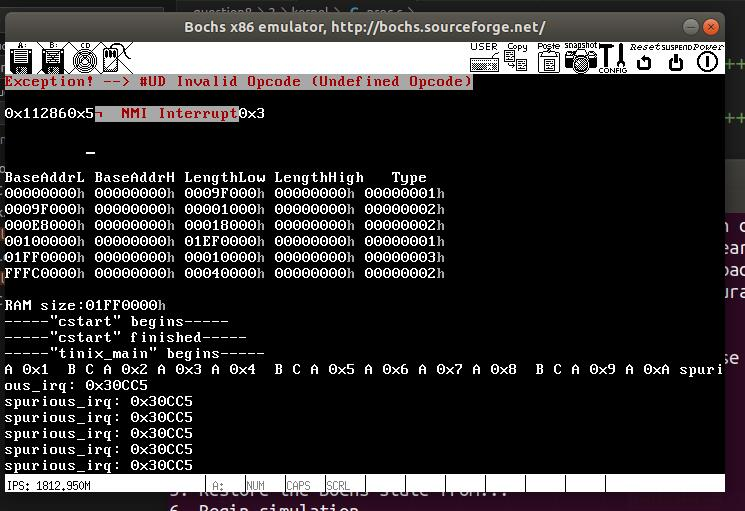
\includegraphics[width=0.8\textwidth]{figures/chapter9/9-3.jpg}
            \caption{系统调用运行结果}
        \end{figure}
优先级调度部分运行结果如下图9-4所示:
        \begin{figure}[H]
            \centering
            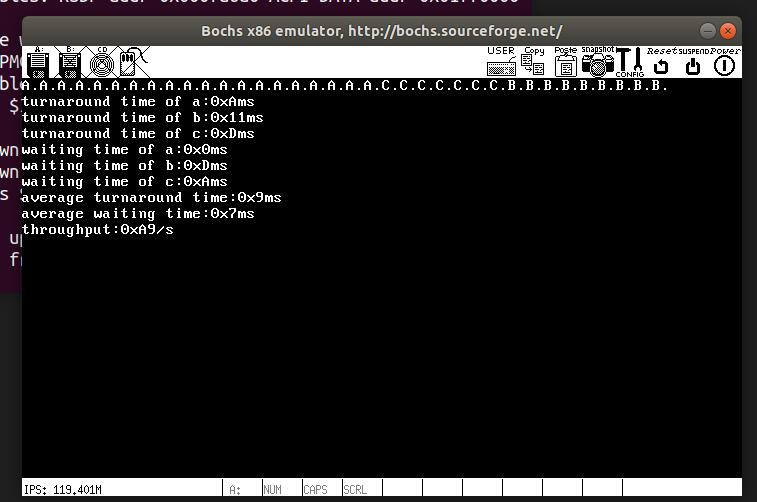
\includegraphics[width=0.8\textwidth]{figures/chapter9/9-4.jpg}
            \caption{优先级调度运行结果}
        \end{figure}
\section{实验总结}
最后的操作系统进阶实验中,首先在内核中添加了一个新的系统调用,该系统调用功能是统计一个进程在执行过程中被调度的次数,然后在用户程序中调用该系统调用。在实现了自定义的系统调用的基础上,我设计了一个简单的进程优先级调度算法。原先的三个进程是无限循环执行的,我将它们的循环次数修改为有限次数。三个进程执行完成后,我计算了它们在优先级调度算法下的周转时间、等待时间以及整个系统的平均周转时间、平均等待时间和吞吐量。通过这次实验,我学会了如何在操作系统中添加自定义的系统调用,熟悉了整个系统调用的流程,并且了解了系统调用的原理和使用方法,同时更深入地理解了进程调度算法的原理和实际应用。\par



\chapter{实验心得体会}\label{cha:latex-brief-intro}

本次操作系统复现实验中,我参考《一个操作系统的实现》\cite{于渊2009orange}这本指导书,将理论知识与实践相结合,复现了一个基本的操作系统。从搭建虚拟机工作环境开始,一步步地实现保护模式和实模式的转换,切换到保护模式之后实加载 Loader 进入内存并将控制权交给 loader,随后将 loader 替换成 kernel 内核,实现进程切换、保存与恢复、调度,并解决可能会出现的中断重入问题。最后实现 I/O 系统,一个由我们自己设计的简单的操作系统就此完成。在这次实验过程中,我通过每一次实验之间代码的不同以及最后呈现的效果的区别,对不同代码对应的操作系统的基本结构、原理和功能有了更清晰明确的理解,也对NASM汇编语言有了初步的认识。\par
这次实验首先深化了我对操作系统的理解。我对操作系统的多进程管理、输入输出处理等方面有了更加深刻和直观的认识。通过亲自实践,我认识到了操作系统是如何协调和管理多个进程的执行,如何处理输入输出请求等。
除此之外,我还增加了对 CPU 硬件的了解。实现一个操作系统不可避免地需要与硬件进行交互,而这次实验让我对一些关键芯片有了初步的了解。其中,我对中断控制芯片 8259A、时钟控制芯片 8253 以及键盘控制芯片 8042 有了初步的认识。了解这些芯片的功能和工作原理,让我意识到操作系统是如何与硬件进行通信和控制的。
最后,在这次实验中,我还初步接触了NASM汇编语言,发现与此前学过的x86汇编语言较为类似,在此基础上通过阅读源码对比并实践运行,我逐渐掌握了NASM汇编语言的基本使用方式,以及编写汇编指令来实现特定的功能,与C语言进行混合编译。\par
由于之前的一些科研工作涉及到过Linux系统,这次实验的环境配置部分没有给我带来过多困扰,但在此前我更多地是了解学习Linux系统的相关指令。在这次实验的操作过程中,我开始从原理上深化理解这些指令的意义,这对我的实操能力带来了很大提升。\par
同时,我非常感谢老师的指导和帮助以及提供的参考资料\cite{于渊2009orange}\cite{mit},没有这些内容作为参考,我无法完成这个实验。通过这次实验,我不仅掌握了操作系统的基本原理和实践技能,还培养了解决问题的能力和动手实践的精神。这对我的职业发展和学术研究都具有重要意义。我将继续深入学习操作系统的知识,并将其应用到未来的学习和研究中。



%此处结束正文-------------------------------------------------------------------------------------------------


\include{pages/backmatter} %%%结论

%%%============================================================================================================%%%

%%%=== 参考文献 ========%%%
\cleardoublepage\phantomsection

\bibliographystyle{plain}        % 参考文献样式,  plain,unsrt,alpha,abbrv,chinesebst 等等
\bibliography{ref/refs}



%%%-------------- 附录. 不需要可以删除.-----------


%\appendix

%\include{pages/appendix1}
%\include{pages/appendix2}

%%%-------------- 教师评语评分 ------------------
\begin{teacher}
\thispagestyle{empty}
评语: 
\par
\vspace*{12.5cm}
\hspace*{7.5cm}评分: 
\vspace*{1cm}

\hspace*{7.3cm}评阅人:

\vspace*{0.5cm}

\hspace*{10.1cm}年\hspace*{1cm}月\hspace*{1cm}日

\vspace*{0.5cm}

{\songti \zihao{4} \makebox[1cm][s]{(备注:对该实验报告给予优点和不足的评价,并给出百分制评分。)}}

\end{teacher}


\cleardoublepage
\end{document}





